%% bare_conf_compsoc.tex
%% V1.4b
%% 2015/08/26
%% by Michael Shell

\documentclass[conference,compsoc]{IEEEtran}

\newcommand {\be}{\begin{equation}}
\newcommand {\ee}{\end{equation}}
% *** MISC UTILITY PACKAGES ***
%
\usepackage{ifpdf}
% Heiko Oberdiek's ifpdf.sty is very useful if you need conditional
% compilation based on whether the output is pdf or dvi.
% usage:
% \ifpdf
   % pdf code
% \else
%   % dvi code
% \fi
\usepackage{verbatim}
% *** CITATION PACKAGES ***
%
\ifCLASSOPTIONcompsoc
  % IEEE Computer Society needs nocompress option
  % requires cite.sty v4.0 or later (November 2003)
  \usepackage[nocompress]{cite}
\else
  % normal IEEE
  \usepackage{cite}
\fi

% *** GRAPHICS RELATED PACKAGES ***
%
\ifCLASSINFOpdf
   \usepackage[pdftex]{graphicx}
  % declare the path(s) where your graphic files are
  \graphicspath{{../ICIP2016/Figs/}}
  % and their extensions so you won't have to specify these with
  % every instance of \includegraphics
   \DeclareGraphicsExtensions{.pdf,.jpeg,.png}
\else
  % or other class option (dvipsone, dvipdf, if not using dvips). graphicx
  % will default to the driver specified in the system graphics.cfg if no
  % driver is specified.
   \usepackage[dvips]{graphicx}
  % declare the path(s) where your graphic files are
   \graphicspath{{../ICIP2016/Figs/}}
  % and their extensions so you won't have to specify these with
  % every instance of \includegraphics
   \DeclareGraphicsExtensions{.eps}
\fi


% *** MATH PACKAGES ***
%
\usepackage{amsmath}


% IEEEtran contains the IEEEeqnarray family of commands that can be used to
% generate multiline equations as well as matrices, tables, etc., of high
% quality.


% *** SUBFIGURE PACKAGES ***
%\ifCLASSOPTIONcompsoc
%  \usepackage[caption=false,font=footnotesize,labelfont=sf,textfont=sf]{subfig}
%\else
%  \usepackage[caption=false,font=footnotesize]{subfig}
%\fi

% *** FLOAT PACKAGES ***
%
%\usepackage{fixltx2e}
% fixltx2e, the successor to the earlier fix2col.sty, was written by
% Frank Mittelbach and David Carlisle. This package corrects a few problems
% in the LaTeX2e kernel, the most notable of which is that in current
% LaTeX2e releases, the ordering of single and double column floats is not
% guaranteed to be preserved. Thus, an unpatched LaTeX2e can allow a
% single column figure to be placed prior to an earlier double column
% figure.
% Be aware that LaTeX2e kernels dated 2015 and later have fixltx2e.sty's
% corrections already built into the system in which case a warning will
% be issued if an attempt is made to load fixltx2e.sty as it is no longer
% needed.
% The latest version and documentation can be found at:
% http://www.ctan.org/pkg/fixltx2e


%\usepackage{stfloats}
% stfloats.sty was written by Sigitas Tolusis. This package gives LaTeX2e
% the ability to do double column floats at the bottom of the page as well
% as the top. (e.g., "\begin{figure*}[!b]" is not normally possible in
% LaTeX2e). It also provides a command:
%\fnbelowfloat
% to enable the placement of footnotes below bottom floats (the standard
% LaTeX2e kernel puts them above bottom floats). This is an invasive package
% which rewrites many portions of the LaTeX2e float routines. It may not work
% with other packages that modify the LaTeX2e float routines. The latest
% version and documentation can be obtained at:
% http://www.ctan.org/pkg/stfloats
% Do not use the stfloats baselinefloat ability as the IEEE does not allow
% \baselineskip to stretch. Authors submitting work to the IEEE should note
% that the IEEE rarely uses double column equations and that authors should try
% to avoid such use. Do not be tempted to use the cuted.sty or midfloat.sty
% packages (also by Sigitas Tolusis) as the IEEE does not format its papers in
% such ways.
% Do not attempt to use stfloats with fixltx2e as they are incompatible.
% Instead, use Morten Hogholm'a dblfloatfix which combines the features
% of both fixltx2e and stfloats:
%
% \usepackage{dblfloatfix}
% The latest version can be found at:
% http://www.ctan.org/pkg/dblfloatfix


% *** PDF, URL AND HYPERLINK PACKAGES ***
%
%\usepackage{url}
% url.sty was written by Donald Arseneau. It provides better support for
% handling and breaking URLs. url.sty is already installed on most LaTeX
% systems. The latest version and documentation can be obtained at:
% http://www.ctan.org/pkg/url
% Basically, \url{my_url_here}.

% correct bad hyphenation here
\hyphenation{op-tical net-works semi-conduc-tor}

% Definitions.
% --------------------
\def\B{{\mathbf B}}
\def\M{{\mathbf M}}
\def\I{{\mathbf I}}
\def\mcT{{\mathcal{T}}}
\def\mcD{{\mathcal{D}}}
\def\mcA{{\mathcal{A}}}
\def\mcL{{\mathcal{L}}}
\def\mcV{{\mathcal{V}}}
\def\p{{\mathbf p}}
\def\q{{\mathbf q}}
\def\r{{\mathbf r}}
\def\s{{\mathbf s}}
\def\S{{\mathbf S}}
\def\mcN{{\mathcal{N}}}
\DeclareMathOperator*{\argmax}{arg\,max} 

\begin{document}
%
% paper title
\title{A Salient Region Detector for Structured Images}


% author names and affiliations
% use a multiple column layout for up to three different
% affiliations
\author{\IEEEauthorblockN{Elena Ranguelova}
\IEEEauthorblockA{Netherlands eScience Center\\
Amsterdam, The Netherlands\\
Email: E.Ranguelova@esciencecenter.nl}
}

% make the title area
\maketitle

% As a general rule, do not put math, special symbols or citations
% in the abstract
\begin{abstract}
Finding correspondences between two images of the same scene or object, taken from different viewpoints and in different conditions, is a challenging task. Furthermore, in the analysis of scientific imagery, it must be possible in terms of human perception to appreciate detected local features, thus making the task even more complex.
\begin{comment} One method, used by ecologists in their population studies and conservation efforts, is photo identification. In addition to identifying individual plants or animals or classifying species, precise phenotypic (appearance) measurements are needed. 
\end{comment}
A renowned generic feature detector, Maximally Stable Extremal Regions (MSER), performs very well on structured images, but has difficulties with blur, lighting and increased resolution. The detected regions do not always correspond to semantically meaningful image structures, and the large number of regions hampers scalability. This paper proposes a Data-driven Morphology Salient Regions (DMSR) detector which overcomes these limitations. We present a new binarization algorithm which uses a threshold derived from the data; the resulting binary image is analyzed for saliency using morphology. DMSR shows transformation invariance and comparable repeatability to MSER on several evaluation benchmarks while obtaining better invariance to lighting, blur and resolution. This is achieved via significantly fewer regions, leading to better scalability. Preliminary results on animal and plant images indicate that DMSR could %indeed 
be a suitable approach for wild-life biometric applications as the detected regions correspond well to the semantic %salient 
image structures. We also introduce OxFrei - a dataset for transformation-independent detection evaluation. 

\end{abstract}

% no keywords




% For peer review papers, you can put extra information on the cover
% page as needed:
% \ifCLASSOPTIONpeerreview
% \begin{center} \bfseries EDICS Category: 3-BBND \end{center}
% \fi
%
% For peerreview papers, this IEEEtran command inserts a page break and
% creates the second title. It will be ignored for other modes.
\IEEEpeerreviewmaketitle


\section{Introduction}
% no \IEEEPARstart
\label{sec:intro}
The first fundamental step in numerous computer vision applications (such as wide baseline stereo matching, image retrieval and visual mining) is to reliably and repeatedly find correspondence between a pair of different images of the same scene or object \cite{Matas2002BMVC, Rodriguez2013, EscaleraCVPR07}. One class of methods, {\em region detectors}, finds salient (distinct) regions, which correspond to the same image patches detected independently in each image. The detectors must be {\em invariant} to usually {\em affine} transformations (e.g.~ viewpoint and scaling) and photometric distortions (e.g.~lighting, blur and resolution). 

\begin{figure}[htb]

\begin{minipage}[b]{.48\linewidth}
  \centering
  \centerline{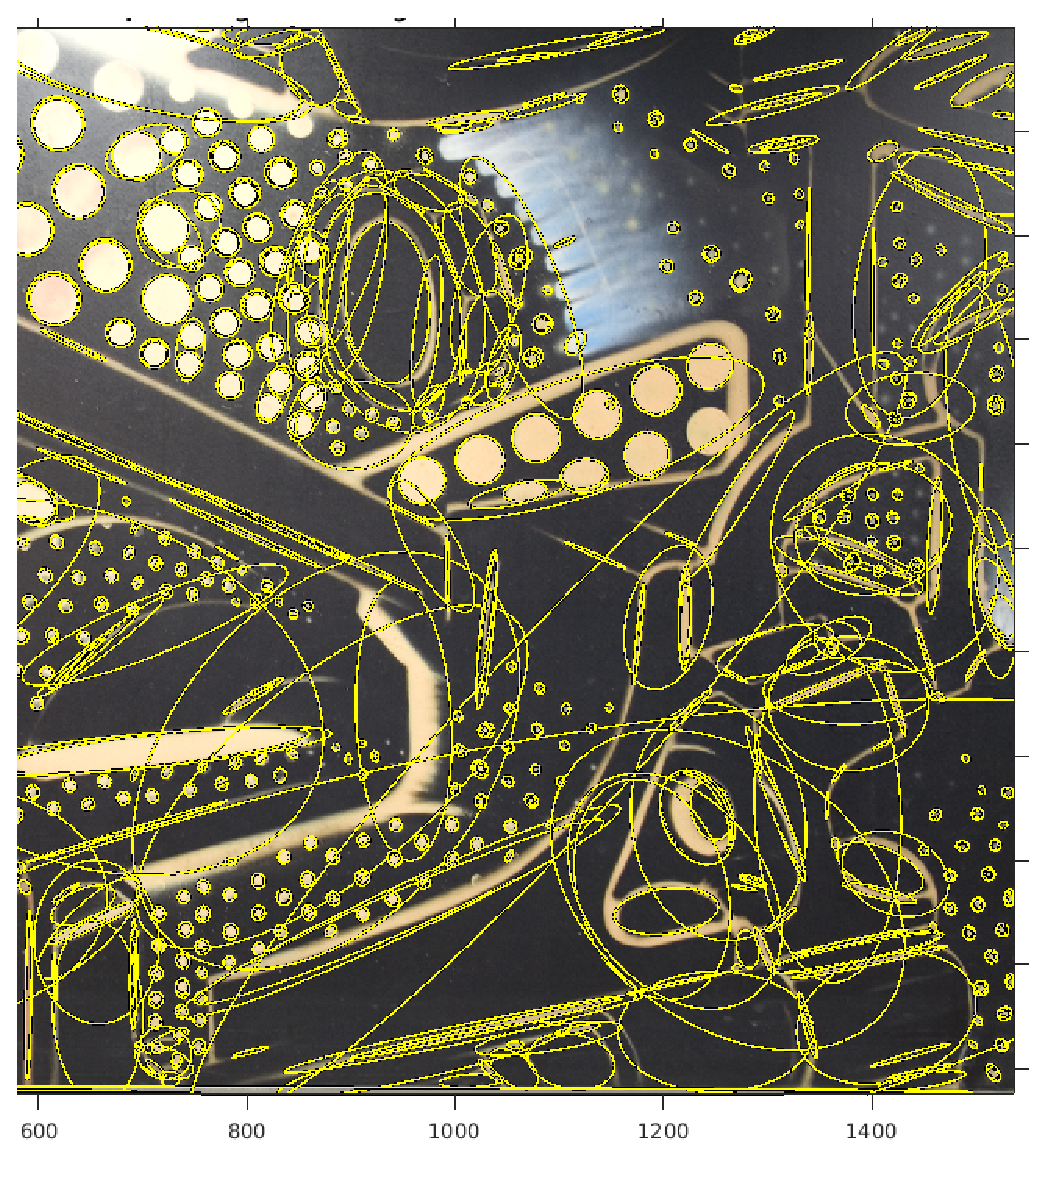
\includegraphics[width=3.8cm]{tnt_mser_lores_zoom}}
\end{minipage}
\begin{minipage}[b]{0.5\linewidth}
  \centering
  \centerline{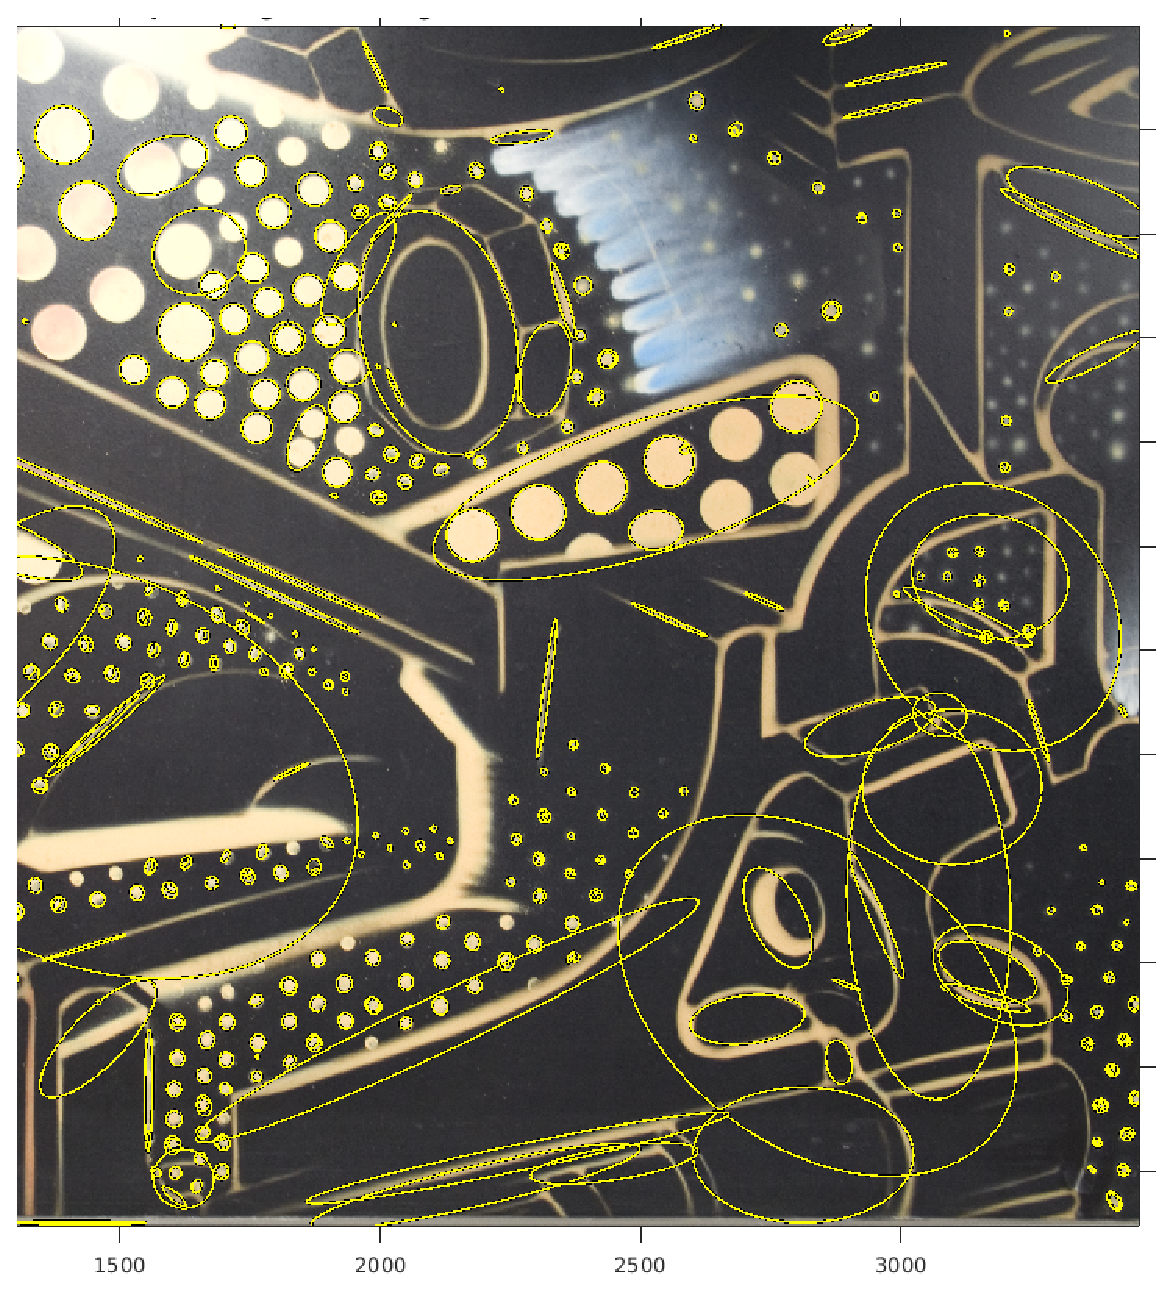
\includegraphics[width=3.8cm]{tnt_mser_hires_zoom}}
\end{minipage}
\hfill
\begin{minipage}[b]{.48\linewidth}
  \centering
  \centerline{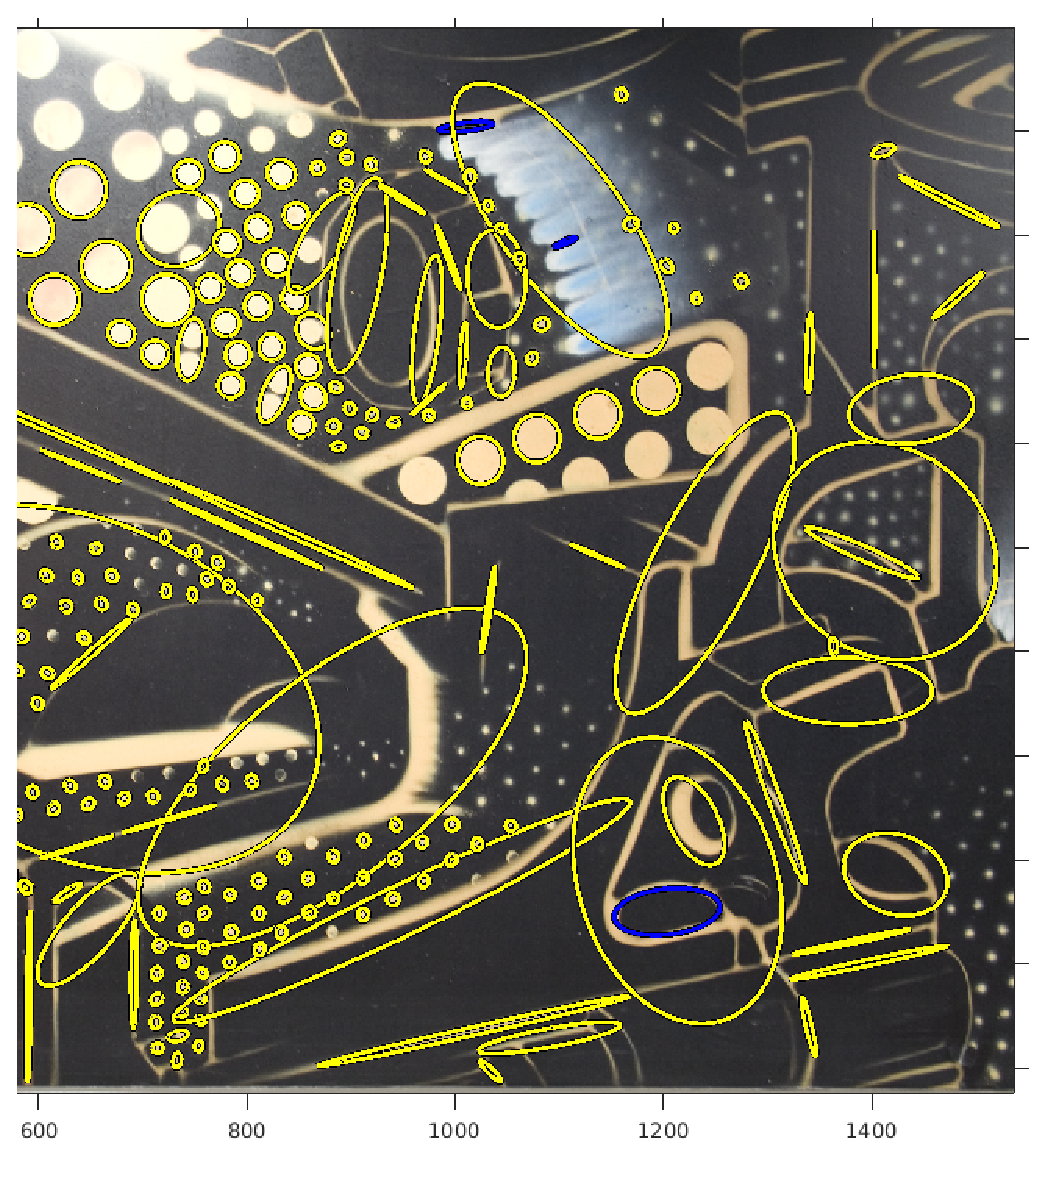
\includegraphics[width=3.8cm]{tnt_dmsr_lores_zoom}}
\end{minipage}
\begin{minipage}[b]{0.505\linewidth}
  \centering
  \centerline{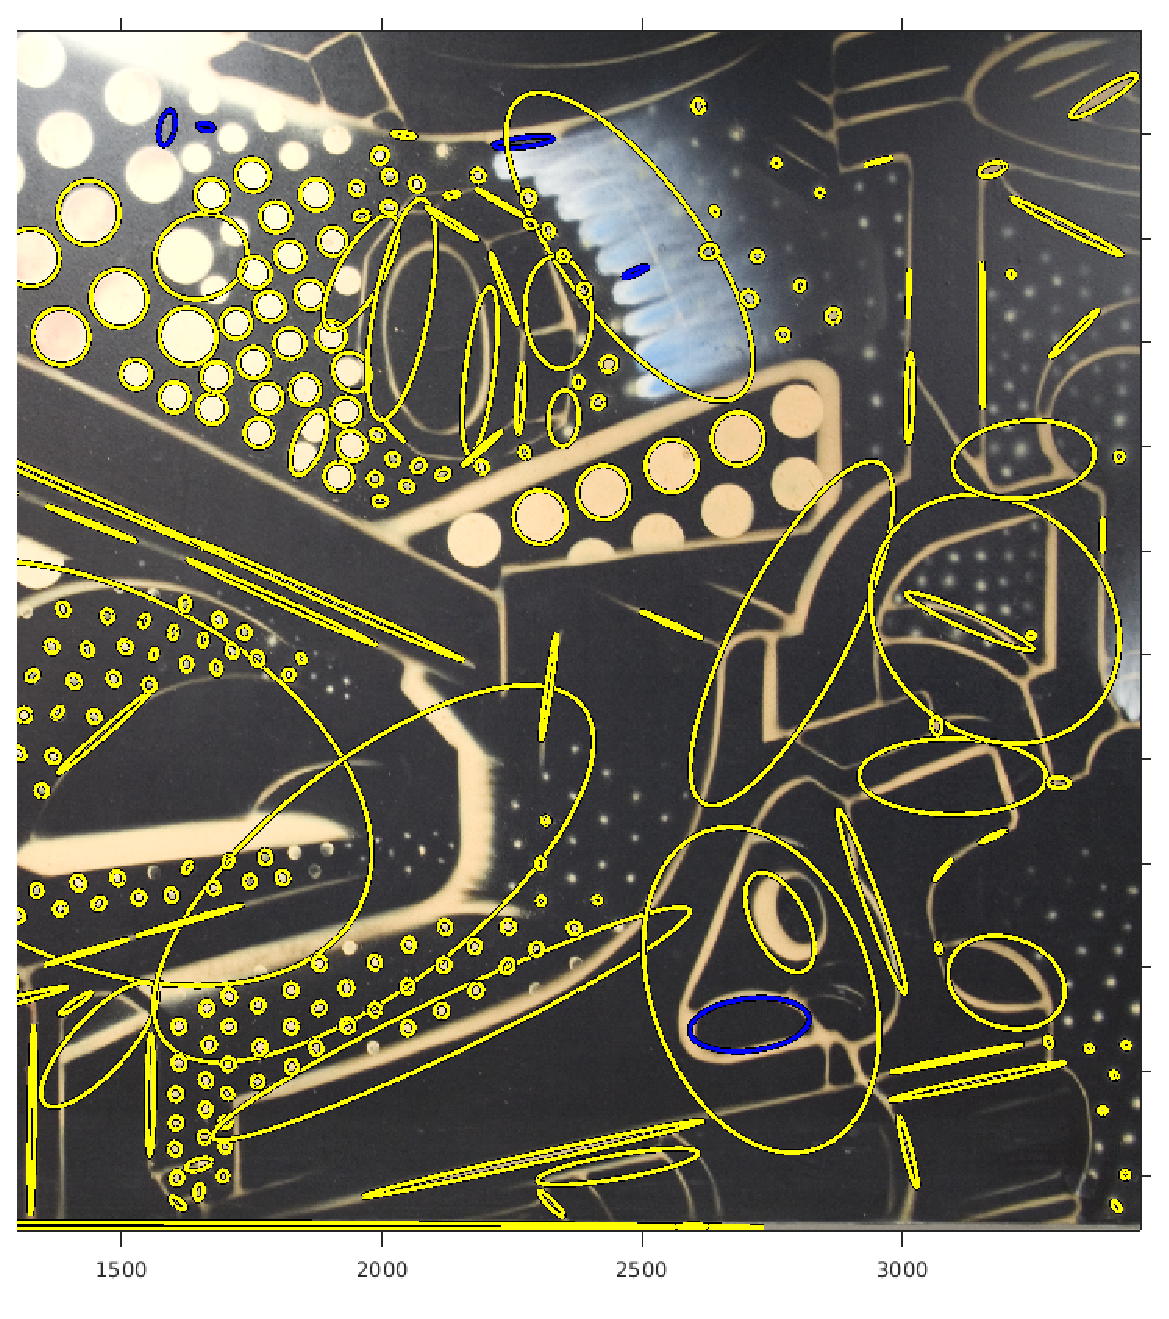
\includegraphics[width=3.8cm]{tnt_dmsr_hires_zoom}}
\end{minipage}
\hfill
\vspace{-0.5cm}
\caption{Region detection on the 'underground' image (detail), TNT dataset.  
Top row: MSER, bottom row: DMSR (proposed detector). Left: low $1.5$~MPixel, right: high $8$~MPixel resolution}
\label{fig:tnt_zoom}
\vspace{-0.4cm}
\end{figure}

A decade ago, a performance evaluation paper by the Visual Geometry Group in Oxford compared existing region detectors \cite{Mikolajczyk:2005}. 
A clear conclusion was that {\em  Maximally Stable Extremal Regions (MSER)} is the best performing detector for {\em structured} scenes, e.g., those containing homogeneous regions with distinctive boundaries \cite{Matas2002BMVC}. MSER has become the de-facto standard in the field: it has been implemented as part of MATLAB, OpenCV, VLFeat, etc. However, despite its success, the detector has several drawbacks: it is sensitive to image blur; it produces nested and redundant regions, and its performance degrades with the increase of image resolution \cite{CorRos2013}. Figure \ref{fig:tnt_zoom} illustrates this degradation in contrast to the robustness to resolution of our proposed {\em Data-driven Morphology Salient Regions (DMSR)} detector on a detail taken from the 'underground' image in the TNT dataset \cite{CorRos2013}. While many of the MSER regions are not found when the image resolution increases from $1.5$~MPixel to $8$~MPixel, the DMSR region detection is consistently resolution invariant. Analyses in geometric scale-space have shown that the formulation of the region stability criterion makes MSER prefer regular shapes \cite{Kimmel11}.


\subsection{Envisioned scientific applications}
While most research has been focused on generic applications, the
 fields of {\em animal and plant biometrics} are attracting more attention \cite{Kuehl2013, leafsnap_eccv2012}. Computer vision is becoming a vital technology enabling the wild-life preservation efforts of ecologists. Along with individual or species photo-identification, scientists wish to obtain reliable measurements of meaningful structures from images. For example, the automated identification of cell structures is one of the new challenges to be met in studies of the structural biology of plants \cite{Quelhas2011}. Analysis of these microscopic features from anatomical sections of wood are very important for studying the secondary growth and development of trees \cite{Brunel2014}. Classifying the cell types can be approached by examining their shape, size and spatial distribution. At the same time, these characteristics are used for automated wood species classification, which is very important to fight illegal logging \cite{Gasson2011}. Therefore, the  automatic detector of regions corresponding to wood cells has to perform well for the two tasks ecology scientists face: identification of species or individuals followed by phenotypic measurements. The generic detectors do not satisfy this need: they produce redundant overlapping regions which often do not coincide with semantic structures (Figures ~\ref{fig:wood}, top and \ref{fig:wood_C}, left).

\subsection{Evaluation benchmarks}
Although crucial for the development of detectors, there is a shortage of region-based evaluation benchmarks, especially for performance analysis that is independent of the image content.  The standard {\em Oxford dataset} is very small: eight test sequences containing six (one base and five transformed) images of the same scene each. Every pair (base, transformed) is related via a given transformation matrix (homography) \cite{Mikolajczyk:2005}.  Each transformation is present only in one test sequence in the structured images and one in the textured images group. The {\em Freiburg dataset} contains $416$ higher resolution images, generated by transforming $16$ base images in order to de-tangle transformations from content \cite{FischerDB14}.  
The {\em TNT dataset} contains versions of the same viewpoint sequences with increasing resolution from $1.5$ to $8$~MPixel per image. Highly accurate image pair homographies are given. This dataset is suitable for evaluating robustness to resolution rather than to transformations \cite{CorRos2013}.  A more resent and larger dataset is the point feature {\em DTU Robot Data Set}, \cite{AanaesDP12}. It  consists of $60$ scenes acquired from $119$ positions (executed with a robotic arm), totaling $135, 660$ color images of a resolution of $1200 \times 1600$. While of a much larger scale and with better precision of correspondences than the Oxford dataset, it is a limited indoor setup and hence does not capture natural outdoor variations of acquisition conditions. Interestingly, the authors report the performance (recall, not repeatability) of MSER on their dataset as only moderate. Also, the image resolutions present in the datasets are still relatively low compared to the demand of the real world digital image applications. 

\subsection{Contributions}
 We propose an integrated solution for both image correspondence and object recognition tasks simultaneously. Our new salient regions detector, DMSR, is related to the {\em Morphology-based Stable Salient Regions (MSSR)} detector that we developed earlier\cite{RangMSSR06, RangHumpb06}. DMRS includes a data-driven binarization that is robust to lighting and blur and yields a much smaller number of regions and is more stable across transformations. It has similar or higher  repeatability (lighting, blur and increased resolution) compared to MSER, while detecting non-redundant perceptually salient regions. DMSR consistently achieves the lowest number of detected regions, which will lead to the best scalability during the following region descriptors matching step.  In addition, we have composed and shared the new OxFrei dataset combining the natural homographies of the Oxford and the higher resolution images of the Freiburg datasets. The dataset has been designed to facilitate transformation-independent detectors performance evaluation. All experimental results, dataset and open-source software are available online to facilitate research repeatability \cite{elena_ranguelova_2016_45156}. 


\section{Related work}
Many researchers have proposed improvements to MSER, but without drastic increase in performance. An MSER color extension, {\em Maximally Stable Color Region}, outperforms both an MSER-per-color-channel combination and a color blob detector \cite{Forssen07}. Improving the MSER region distinctiveness by morphological dilation on the detected Canny edges is proposed in \cite{Wang14}. The improved detector shows better performance in a classification application, but evaluation of repeatability is not reported. 
Chen et al.~also combine MSER with Canny edges to cope with blur for detecting text in natural images \cite{Chen11}.
Kimmel et al. %not only point out the preference of the algorithm towards regular shapes, but also 
propose several reinterpretations of the stability measure to define more informative shape descriptors \cite{Kimmel11}. 

Interesting research has been conducted by Martins et al.~who propose {\em feature-driven} MSER, called  {\em Stable Salient Shapes} (SSS), by extending the concept of stable regions from detection using the original image to one from a boundary-related features enhanced representation \cite{MartinsVisapp12, Martins12}. This is done via ``feature-highlighting'' of edges and ridges generating saliency maps which are used as domains for the MSER detector. As a result, SSS is less sensitive to blurring, but it also detects even more regions per image in comparison to MSER. While the authors consider the latter an improvement, since it decreases the detector's sensitivity to occlusion, we argue that in the context of scaling up or in processing animal biometrics imagery usually obtained with care for minimal occlusion, this is a drawback. Their approach also improves the {\em completeness} of the local features (``the information contained in the image should be preserved by the features as much as possible'' \cite{Dickscheid2011}), \cite{Martins2016OnTC}. The authors claim that the completeness property of SSS makes it a suitable detector to solve object recognition tasks, but their software is not shared.

% PCBR
A region detector suitable for object-class recognition, the {\em Principal Curvature-Based Region (PCBR)}, uses curvilinear structures (ridges) to enhance the regions \cite{DengZMDS07}. PCBR differs from MSER in two aspects: it analyses regions in scale space, thus providing different levels of region abstraction, and it also overcomes the problems caused by local variations within regions by focusing on their boundaries rather than interiors. PCBR is similar to our approach in using morphological operators for detecting robust watershed regions, but this is done on the principal curvature image instead of on the intensity (or binarized) image. The reported average repeatability on the Oxford dataset is worse than that of MSER given that PCBR has been designed for object-class recognition. PCBR in combination with object-class recognition algorithms has been able to distinguish between two related species of stone-fly larvae with very similar appearance. The comparison, however, is with Kadir's salient detector \cite{Kadir2004} and Hessian-affine, not with MSER.  Dzeng et al.~point out the importance of designing detectors tailored to object recognition tasks separately from the detectors designed for general applications like wide-baseline stereo matching (such as MSER). Our aim is, however, to addresses both applications with the same technology.

%%%%%%%%%%%%%%%%%%%%%%%%%%%%%%%%%%%%%%%%%%%%%%%%%%%%%%%%%%%%%%%%%%%%%%%%%%%%%%%%%%%%%%%%%%%%%%%%%%%%%%%%%%%%%%%%%%%%%%%%%%%%%%%%%%%%%%%%%%%%%%%%%%%%%%%%%%%%%%%%%%%%%%%%%
\section{Data-driven Morphology Salient Regions Detection}
\label{sec:DMSR}


MSER decomposes a gray-scale image into binary cross-sections and evaluates the stability of the connected components across sections to determine maximally stable regions. In contrast, DMSR starts with a data-driven binarization. The single binary image is then analyzed for saliency using binary morphology. %Thus, the problem of salient region detection is transformed into binary saliency.

\subsection{Binary Salient Regions Detection}
\label{ssec:binary}
We claim that the perceptual saliency in a binary image of a structured scene 
 $\B: \mcD \subset \mathcal{Z}^2 \rightarrow \{0,1\}$ (1-white, 0-black)
is only due to the spatial layout of the image regions. 
There are $4$ types of salient regions grouped into: {\em Inner Salient Structures (ISS)} and {\em Boundary Salient Structures (BSS)}. The $2$ types of ISS are (1) {\em holes} -- set of connected black pixels entirely surrounded by white pixels, and (2) {\em islands} -- set of connected white pixels surrounded by black ones, i.e.~the inverse of holes. A significant connected component (CC) ${\cal B}^1$ is defined as a CC with area proportional to the image area by $\Lambda$.
The $2$ BSS are (3) {\em protrusions}- set of white pixels on the border of a significant CC, which if pinched off from the CC will increase its boundary with no more than $2\pi r$, where $r$ is the radius of the morphological structuring element (SE), and (4) the {\em indentations}- protrusions inverse. 
These types, defined in Table \ref{table:binary_sal}, also apply to the MSSR detector \cite{RangHumpb06}. 

The regions are obtained from $\B$ by morphological operations \cite{Soille}. 
%holes
The {\em hole filling} operation $\bullet (\cdot)$ on the set of all white pixels $\B ^1$ intersected with the set of all black pixels $\B^0$ can be used to detect holes:
\be
S^i_{01} = \rho^i_{01}(\B)= \bullet(\B ^1) \cap \B^0 \label{eqn:sal:inn:01}.
\ee

%----------------------------------------------------------------------
\begin{table}[hbt]
%\vspace*{-0.4cm}
\caption{Binary saliency definitions used in Section \ref{ssec:binary}.}\label{table:binary_sal}
\begin{minipage}[b]{0.99\linewidth}\begin{tabular}{|l l|}
\hline
{\bf ISS} & A CC $S^i_{fb} = \{\p \in \mcD, \forall \p=foreground,$\\&$\forall \q \in \partial S^i_{fb}, \q=background, \q \notin \partial \B $ \},\\
$2$ types & $S^i_{10}$ (islands), $S^i_{01}$  (holes); $\S^i = S_{01}^i \cup S_{10}^i$\\
{\bf BSS} &  $S_{fb}^b: \{\p \in S_{fb}^b \subset{\cal B}^f, \forall \p = foreground,$\\&$ \q \in \partial S_{fb}^b \subset {\partial \cal B}^f,\forall \q = background \}$, \\
& $|\partial {\cal B}^f| - |\partial ({\cal B}^f \backslash S_{fb}^b)| < 2 \pi r$\\
$2$ types & $S^b_{10}$ (protr.), $S^b_{01}$ (indent.); $\S^b = S_{01}^b \cup S_{10}^b$\\
{\bf Regions} &  $\S = \S^i$ (DMSR); $\S = \S^i \cup \S^b$ (DMSRA)  \\
\hline
\end{tabular}
%\hfill
\centering
\end{minipage}
%\vspace*{-0.4cm}
\end{table}

%islands
Islands can be obtained either similarly but from the inverted image or by identifying all non-significant CCs:
\be
S^i_{10} = \rho^i_{10}(\B)= \bullet(\B ^0) \cap \B^1 = \B^1 \backslash \bigcup_j{{\cal B}_j^1} \label{eqn:sal:inn:10}.
\ee

The morphological {\em opening} operator (based on SE
$E$- disk with radius $r$)  $\gamma_E(\B)$ generally smooths a CC's contour 
eliminating thin protrusions. As a consequence, protrusions can be obtained by subtracting an opened CC from the original (this is known as the {\it white tophat
transform} $WTH_E(\B) = \B - \gamma_E(\B)$):
\be
S^b_{10} = \rho^b_{10}(\B)=   \bigcup_j WTH_E({\cal B}_j^1) \label{eqn:sal:bor:10}.
\ee
Morphological {\em closing} $\phi_{E}(\B)$ tends to narrow breaks and long thin indentations.
Therefore, indentations can be picked up by applying the {\em black top hat (BTH)} transform  $BTH_E(\B) = \phi_E(\B) - \B$:
\be
S^b_{01} = \rho^b_{01}(\B)=  \bigcup_j BTH_E({\cal B}_j^1) \label{eqn:sal:bor:01}
\ee
or by applying the WTH to the inverted image.

The binary saliency operator $\rho$ is therefore defined via:
\be
\rho = \gamma_\lambda \circ (\rho^i_{01} \cup\rho^i_{10} \cup
\rho^b_{01} \cup \rho^b_{10}),
\ee
where the  {\em area opening} operator  $\gamma_{\lambda}$ removes isolated regions smaller than $\lambda$ pixels.
\begin{comment}
The hole-filling operation does not depend on the size of the SE, therefore the ISS can be detected as affine covariant regions.
This is not the case for the scale-invariance of the detected BSS. 
We propose choosing a small $r$ which also minimizes the inaccuracy of maximum $2 \pi r$ along the ``disconnection boundary''
$\partial ({\cal B}^f \backslash S_{fb}^b)$. All detected salient regions $\S$ have accurate boundaries as there is no smoothing involved.
\end{comment}

 Figure \ref{fig:binary_sal} illustrates the exact shaped binary salient 
regions detected from a synthetic $100 \times 100$ binary image with DMSR parameters $\Lambda=1/100$, $r=5$ and $\lambda = 10$. 

\begin{figure}[htb]
\vspace{-0.2cm}
\begin{minipage}[b]{.49\linewidth}
  \centering
  \centerline{
\includegraphics[width=5cm]{binary_marks}}

\end{minipage}
%\hfill
\begin{minipage}[b]{0.49\linewidth}
  \centering
  \centerline{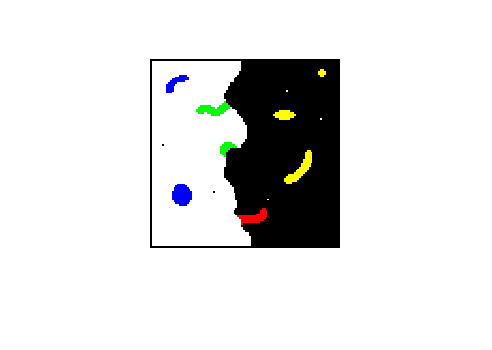
\includegraphics[width=5cm]{binary_marks_clean_color_coded}}

\end{minipage}
\vspace{-0.3cm}
\caption{Binary salient regions detection.
Color coding: ISS: holes - blue, islands - yellow; BSS:
indentations - green, protrusions - red.}
\label{fig:binary_sal}
\end{figure}

The ISS are similar to the definition of the MSER+ and MSER- regions \cite{Matas2002BMVC}. While MSER detects both types, DMSR (and MSSR) is parametrised with the desired type(s) of salient regions to look for. In this paper, detectors using only ISS, i.e., directly comparable to MSER, are denoted by DMSR/MSSR, while DMSRA/MSSRA are detectors using all region types.
%----------------------------------------------------------------------

\subsection{Data-driven binarization}
\label{ssec:binarize}
Any gray-scale image  $\I:~\mcD~\subset~\mathcal{Z}^2~\rightarrow ~\mcT $, where $\mcT=\{0,1,\ldots, t_{max}\}$ and $t_{max}=255$ is the maximum gray value $2^n-1$ encoded by $n=8$ bits, can be decomposed into cross-sections at
every possible level $t$:  $\I = \sum_{t \in \mcT}CS_t(\I)$. Obtaining a section at level $t$ is equivalent to thresholding the image at threshold $t$: $CS_t(\I)= 1.(\I>t) + 0.(\I<t)$ is a binary image. 

Both MSER and MSSR need multiple binary cross-sections: the former uses minimum area change of a CC as stability criteria, while the latter generates cumulative binary saliency masks to determine salient regions. In this paper we argue that it is possible to obtain a single optimum binarization inspired by the notion of feature completeness \cite{Dickscheid2011}. Along with robustness (invariance to transformations), speed (detection should be fast) and sparseness (features should be less than the image itself), an important prerequisite for a good detector is completeness - the salient information present in an image should be maximally preserved. We argue that for a detector which should also reflect saliency, preserving a maximum number of CCs is a way of achieving completeness. On the other hand, larger (significant) CCs are perceptually more salient than smaller CCs. 

We define, then, three sets of connected components in $CS_t(\I)$: $\mcA_t$- {\em all}, $\mcL_t$- the {\em large} and $\mcV_t$- the {\em very large} CCs.  The CC size in the last two categories are defined by $\Lambda_{\mcL}$ and $\Lambda_{\mcV}$ fraction of the image area $A_{\I}$. Let us denote the normalized number of elements in a set ($|\cdot|$) by $\Vert \cdot \Vert = |\cdot| / \max_{t \in \mcT}|\cdot|$.
Finding the optimal binarization threshold $t_{opt}$ is then defined as:
\begin{equation} \label{eq:bin}
\vspace{-0.05cm}
t_{opt} = \argmax_{t \in \mcT}( w^{\mcA} \Vert \mcA_t \Vert + w^{\mcL} \Vert \mcL_t \Vert + w^{\mcV} \Vert \mcV_t \Vert ),
\vspace{-0.05cm}
\end{equation}
where $w^{\cdot}$ are the weights per set of CCs.  

In comparison to the standard Otsu thresholding which does not select a single $CS$ stable across photometric transformations, choosing $t_{opt}$ as defined ensures a transformation-invariant stable number of regions. Figures \ref{fig:binary_hist} and \ref{fig:leuven_bin} show the Otsu and the data-driven thresholding in respect to lighting. When the lighting decreases, the Otsu thresolding produces fewer regions with often smaller extent (e.~g.~the cars' windows), while the proposed binarisation generates regions with the same spatial extent (Fig.~\ref{fig:leuven_bin}). 
%------------------------------------------------------------------------
%\vspace{-0.8cm}
\begin{figure}[htb]

\begin{minipage}[b]{0.99\linewidth}
  \centering
  \centerline{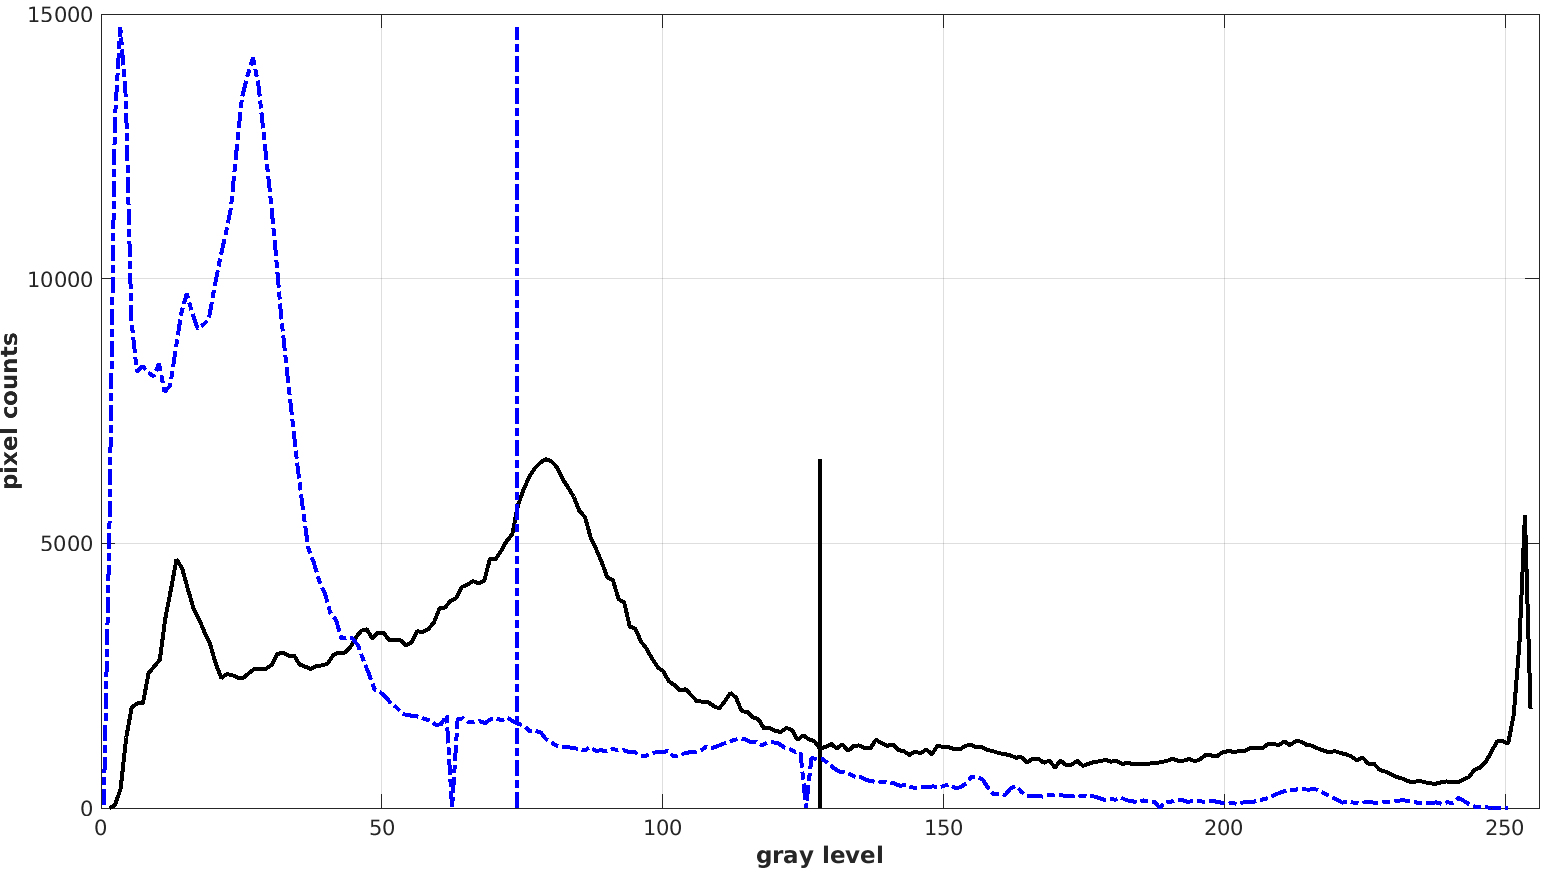
\includegraphics[width=8.5cm]{hist_otsu_leuven_1_4}}
  \centerline{(a) Otsu}\medskip
\end{minipage}
\hfill
%\vspace{-0.5cm}
\begin{minipage}[b]{0.99\linewidth}
  \centering
  \centerline{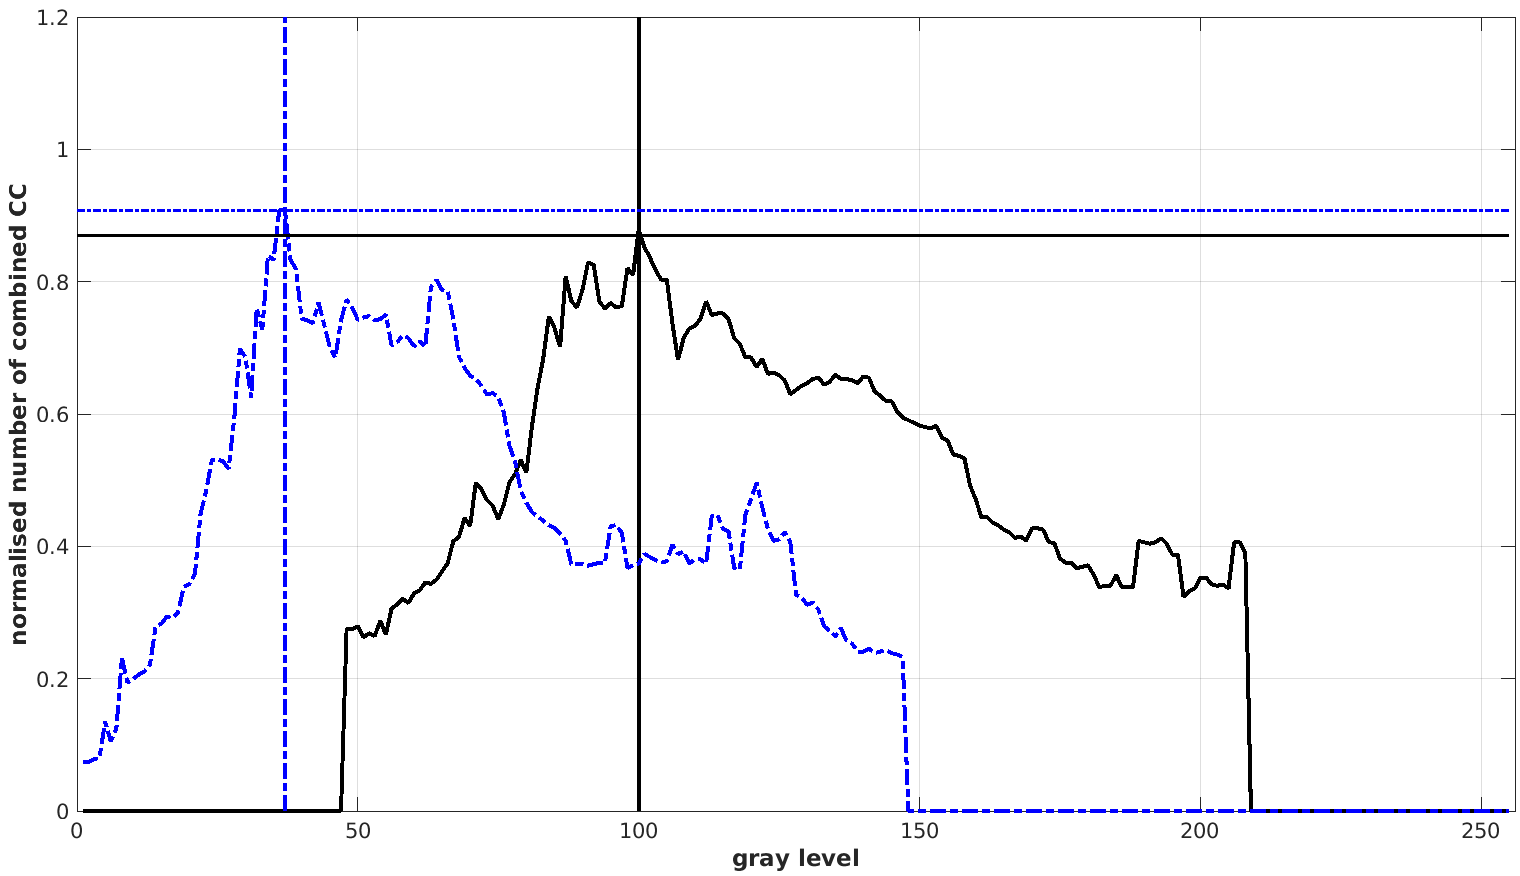
\includegraphics[width=8.5cm]{hist_numcc_leuven_1_4}}
\centerline{(b) Max number CC}\medskip
\end{minipage}
\hfill
%\vspace{-0.5cm}
\caption{Finding the optimal threshold for two images from the 'Leuven' sequence 
(Oxford dataset, lighting): the base image- solid black line, the forth image - dotted blue line.}
\label{fig:binary_hist}
%
\end{figure}
%------------------------------------------------------------------------
%\vspace{-0.5cm}

\begin{figure}[htb]

\begin{minipage}[b]{.48\linewidth}
  \centering
  \centerline{\includegraphics[width=3.5cm]{leuven1}}
%  \vspace{1.5cm}
%   \centerline{(a)}\medskip
\end{minipage}
\hfill
\begin{minipage}[b]{0.48\linewidth}
  \centering
  \centerline{\includegraphics[width=3.5cm]{leuven4}}
%  \vspace{1.5cm}
  % \centerline{(b)}\medskip
\end{minipage}
\hfill
\begin{minipage}[b]{0.48\linewidth}
  \centering
  \centerline{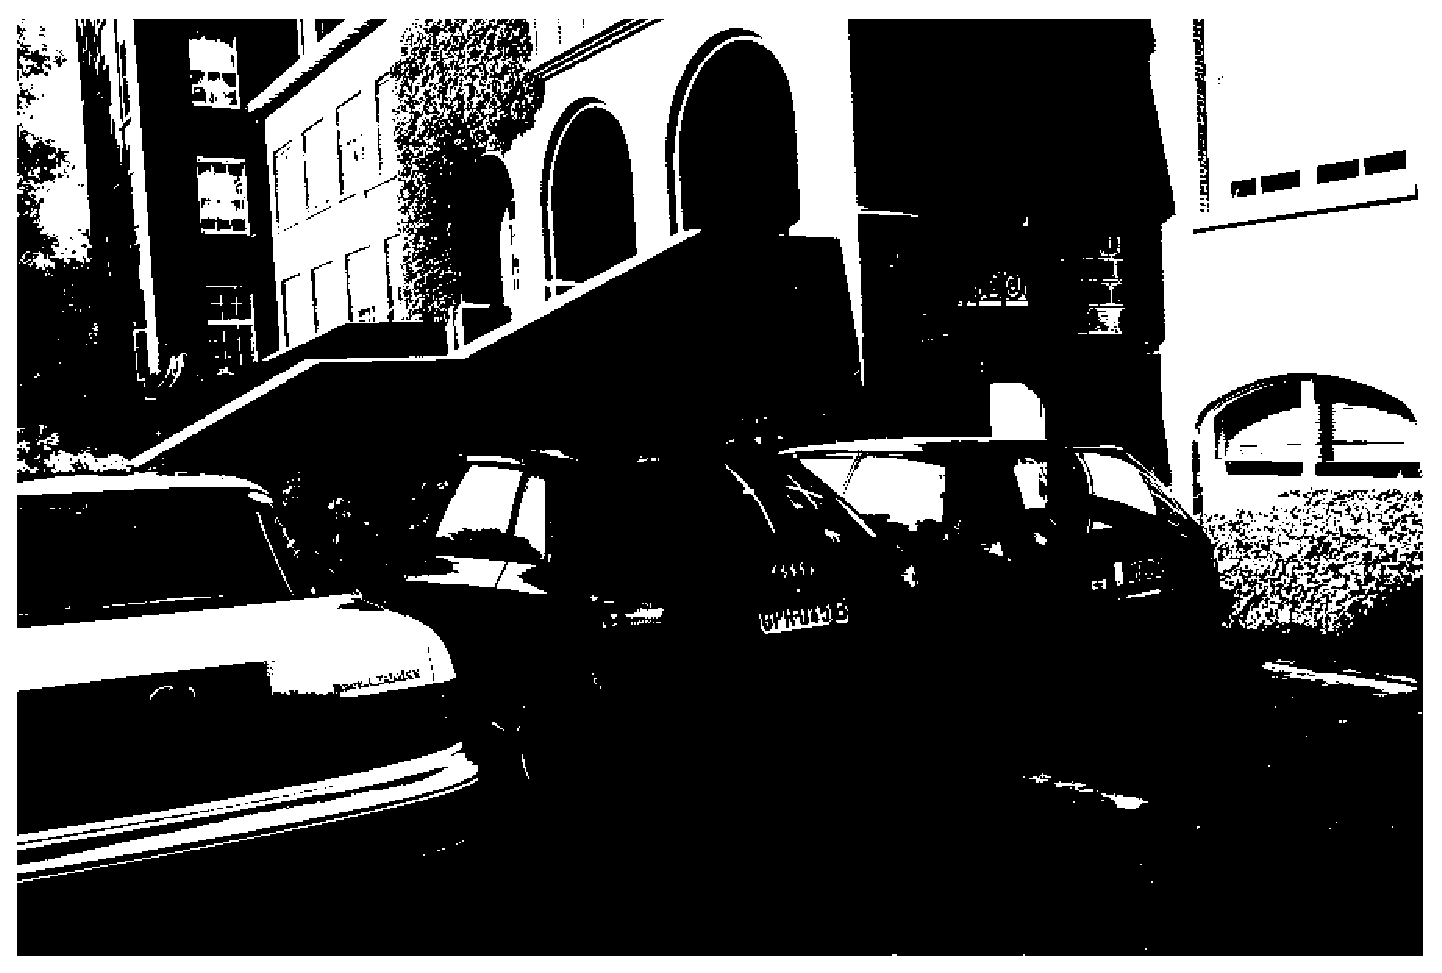
\includegraphics[width=3.5cm]{leuven1_otsu}}
%  \vspace{1.5cm}
  % \centerline{(c)}\medskip
\end{minipage}
\begin{minipage}[b]{.48\linewidth}
  \centering
  \centerline{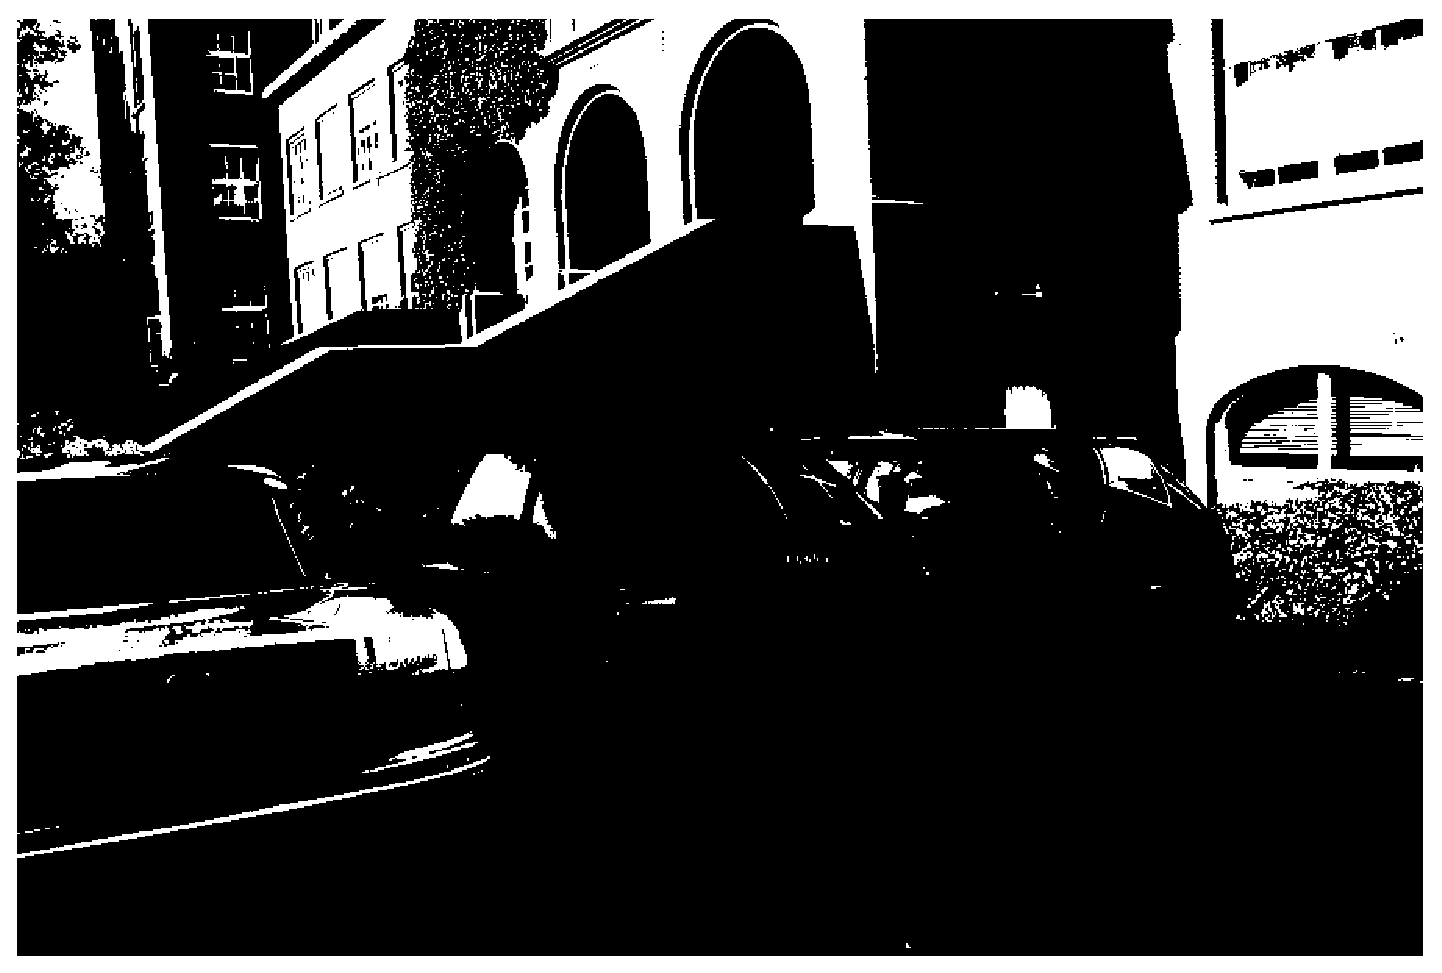
\includegraphics[width=3.5cm]{leuven4_otsu}}
%  \vspace{1.5cm}
%   \centerline{(a)}\medskip
\end{minipage}
\hfill
\begin{minipage}[b]{0.48\linewidth}
  \centering
  \centerline{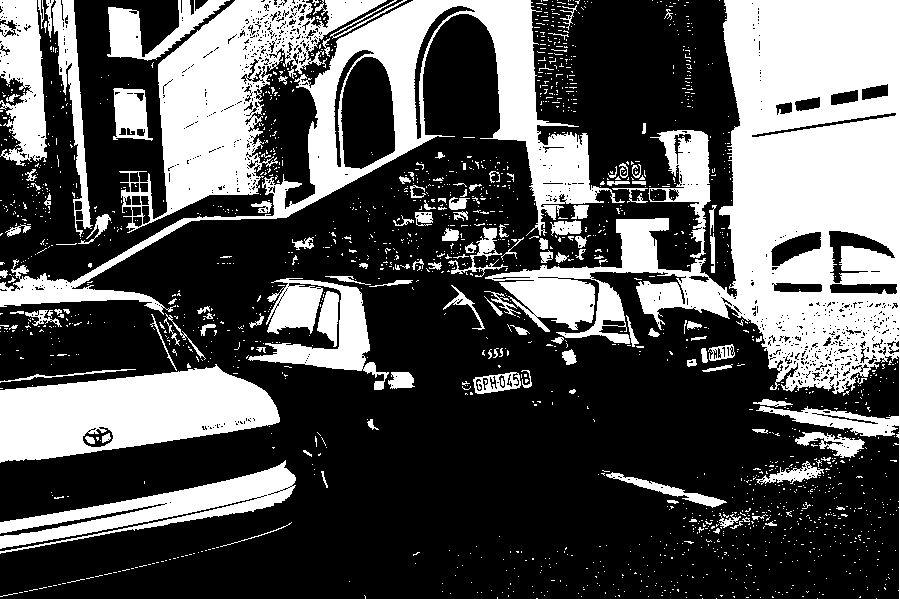
\includegraphics[width=3.5cm]{leuven1_numcc}}
%  \vspace{1.5cm}
%   \centerline{(b)}\medskip
\end{minipage}
\hfill
\begin{minipage}[b]{0.48\linewidth}
  \centering
  \centerline{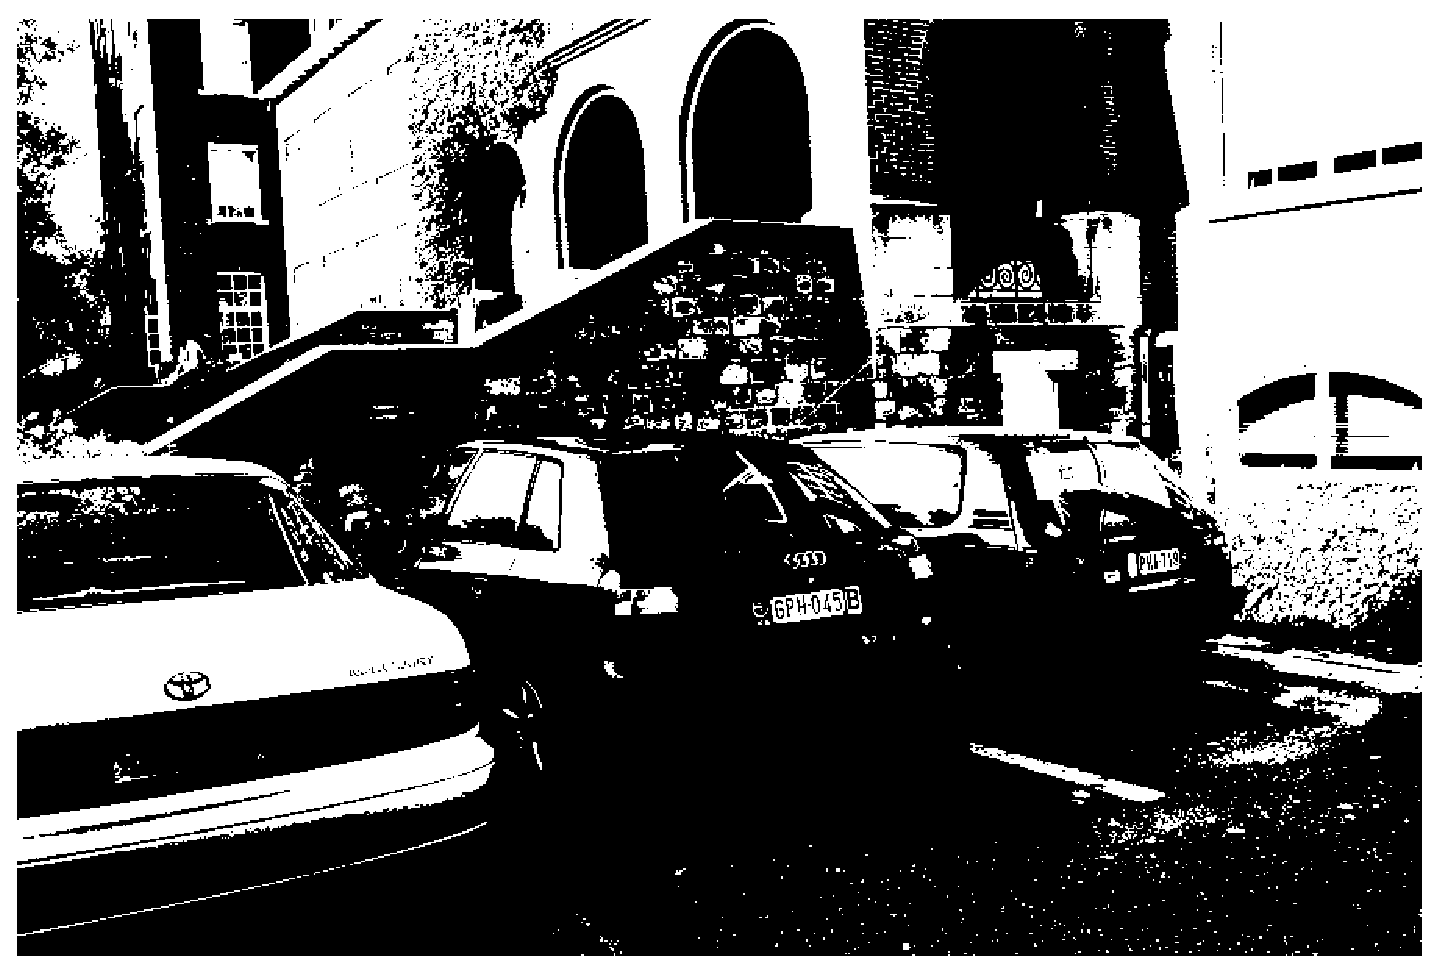
\includegraphics[width=3.5cm]{leuven4_numcc}}
%  \vspace{1.5cm}
%   \centerline{(c)}\medskip
\end{minipage}

 %\vspace{-0.5cm}
\caption{Binarization of two images of the 'Leuven' sequence (lighting). Left: base image, right: forth image;   top row: gray scale; middle row: Otsu binarization, bottom row: proposed binarization.}
\label{fig:leuven_bin}
%
\end{figure}
%------------------------------------------------------------------------

\subsection{DMSR}
After the data-driven binarization, the DMSR detector finds the set of affine-covariant regions $\S$ from the single binary image $CS_{t_{opt}}$ as described in Section \ref{ssec:binary} and \cite{RangMSSR06, RangHumpb06}. As a result, DMSR produces fewer non-overlapping and perceptually salient regions compared to MSER. This is illustrated in Figures \ref{fig:tnt_zoom}, \ref{fig:det_graffiti}, \ref{fig:tails_mser}, \ref{fig:tails_dmsr}, \ref{fig:wood} and \ref{fig:wood_C} where the regions are visualized by their equivalent ellipses, not by their exact detected shapes.

%------------------------------------------------------------------------
\begin{figure}[htb]

\begin{minipage}[b]{.49\linewidth}
  \centering
  \centerline{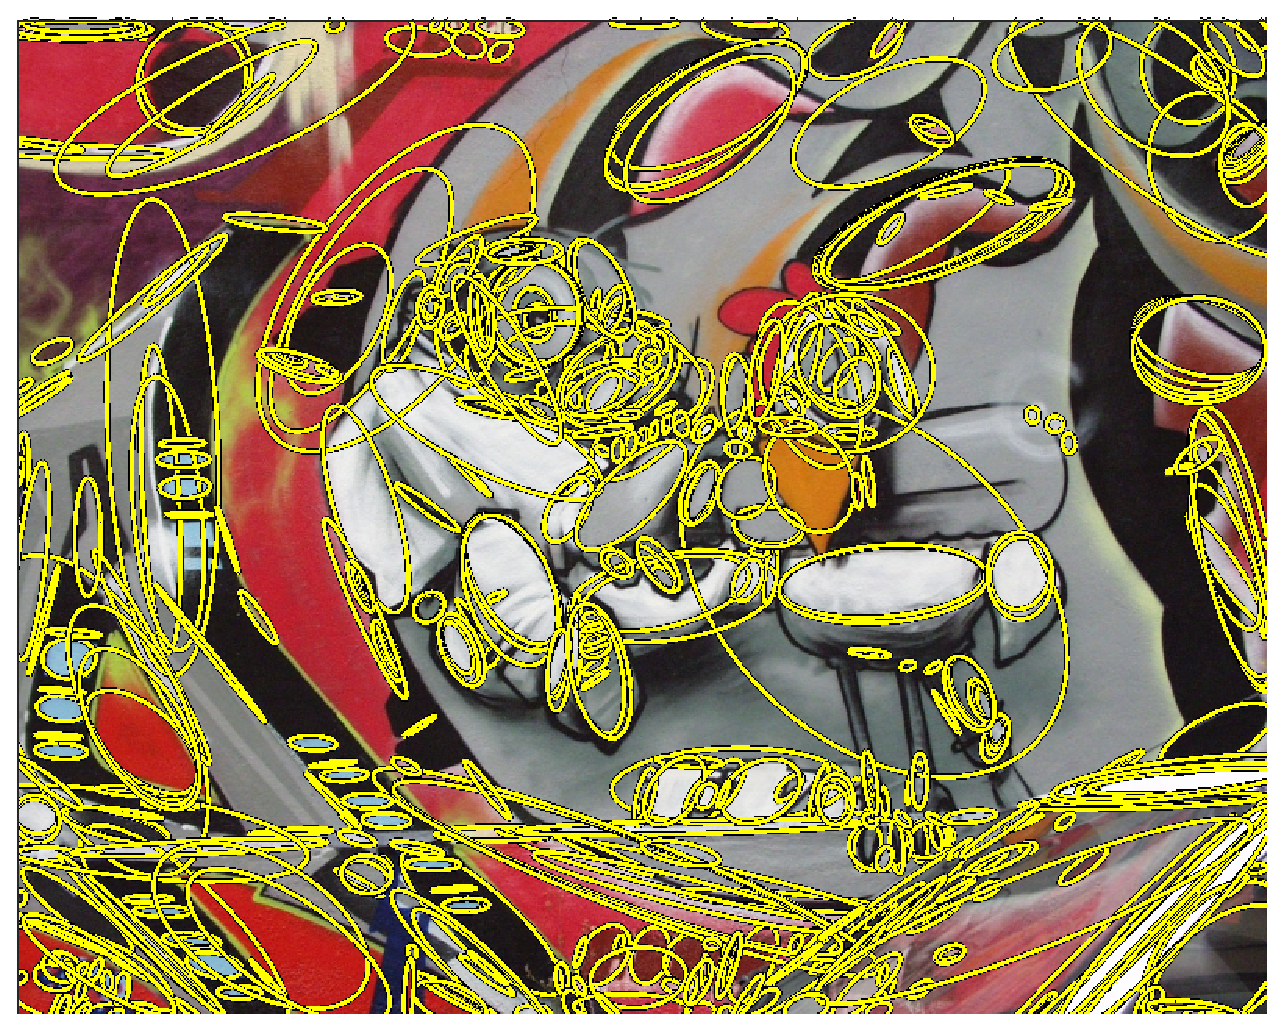
\includegraphics[width=4.0cm]{mserGraffiti1}}
 % \vspace{0.2cm}
 % \centerline{(a) MSER}\medskip
\end{minipage}
\hfill
\begin{minipage}[b]{0.49\linewidth}
  \centering
  \centerline{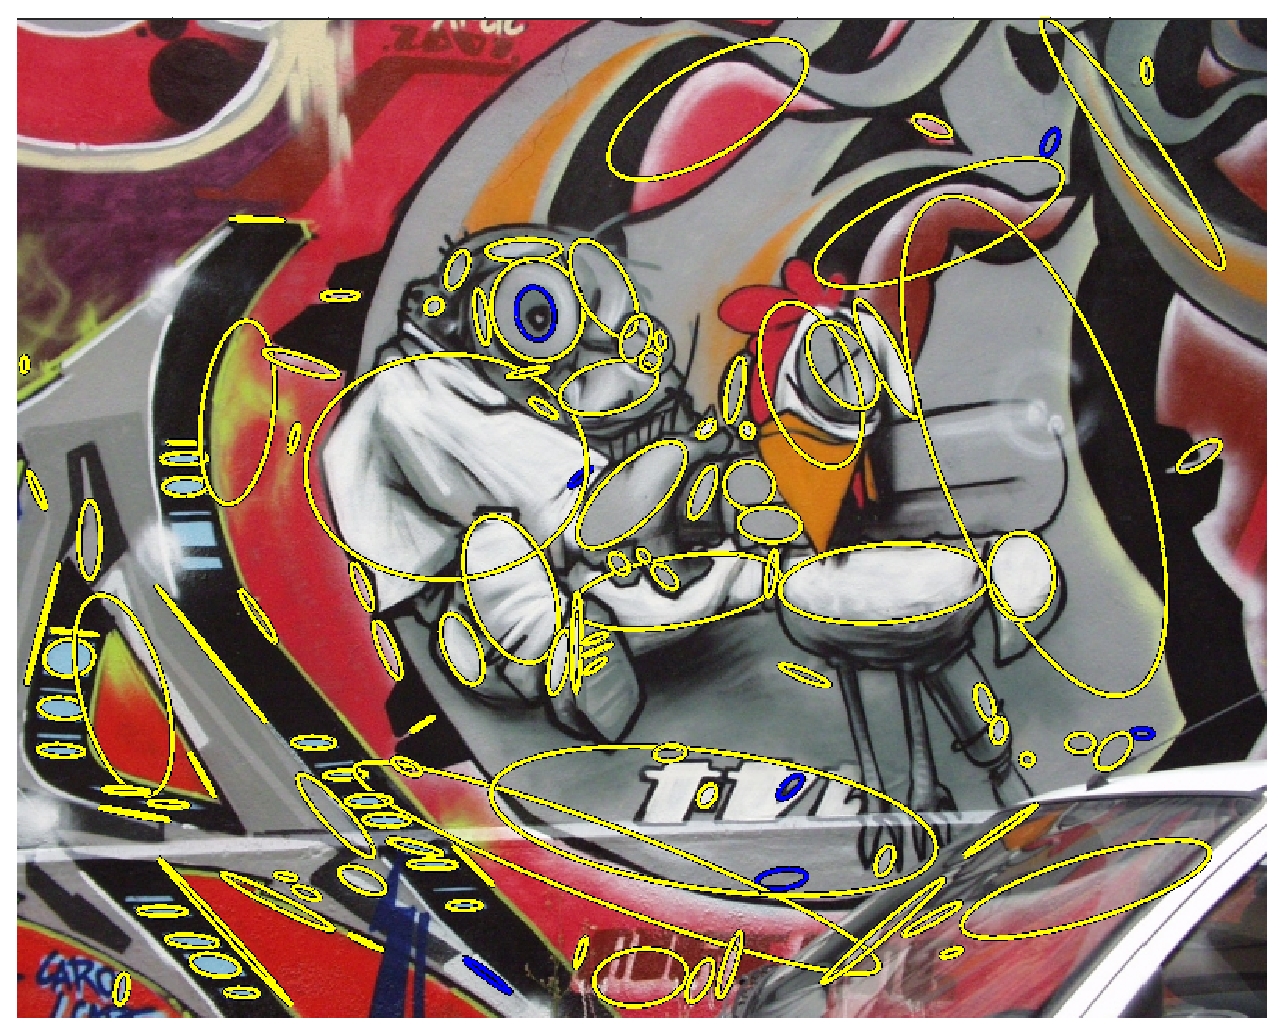
\includegraphics[width=4.0cm]{dmsrGraffiti1}}
 % \vspace{0.2cm}
 % \centerline{(b) DMSR}\medskip
\end{minipage}
\vspace{-0.25cm}
\caption{Region detectors on the base image of the 'Graffiti' sequence, Oxford dataset. Left: MSER, right: DMSR}
\label{fig:det_graffiti}
%
\end{figure}
%%%%%%%%%%%%%%%%%%%%%%%%%%%%%%%%%%%%%%%%%%%%%%%%%%%%%%%%%%%%%%%%%%%%%%%%%%%%%%%%%%%%%%%%%%%%%%%%%%%%%%%%%%%%%%%%%%%%%%%%%%%%%%%%%%%%%%%%%%%%%%%%%%%%%%%%%%%%%%%%%%%%%%%%%
\section{Performance  Evaluation}
\label{sec:perf}


We have applied the standard performance evaluation metrics - the {\em repeatability score} ($R$) and the {\em number of correspondences} ($N_C$) \cite{Mikolajczyk:2005}. The maximum overlap error between matching regions is set to $40\%$ as in \cite{Mikolajczyk:2005}. The repeatability score between a pair of base and transformed image, $(\I_B,\I_T)$, is the ratio between $N_C$ in the part of the images with common content and the minimum number of regions in the image pair. Since we were intrested in finding correspondencies between salient regions from structured images only, we focused on this subset from each dataset and ignored the textured scenes (e.g. 'Trees', 'Bark' etc. from the Oxford dataset). We considered five region detectors for evaluation: MSER, MSSR(A) and DMSR(A). For MSER we used the original Matas software with its default settings and the (D)MSSR(A) parameters are: $r = 0.02*\sqrt{A_{\I} / \pi}$, $\lambda=3r$, $\Lambda_{\mcL}=0.001$, $\Lambda_{\mcV}=0.01$.
All performance plots and detected regions on all data are available online \cite{elena_ranguelova_2016_45156}.

\subsection{Binarization}
In order to determine the binarization weights from equation (\ref{eq:bin}), we have tested all possible meaningful combinations of weights ($\sum w^{\cdot} =1, w^{\cdot} \in [0.1,0.6] $) for the sequences of the Oxford dataset.
%------------------------------------------------------------------------
\begin{figure}[htb]
\centering
\begin{minipage}[b]{.99\linewidth}
  \centering
  \centerline{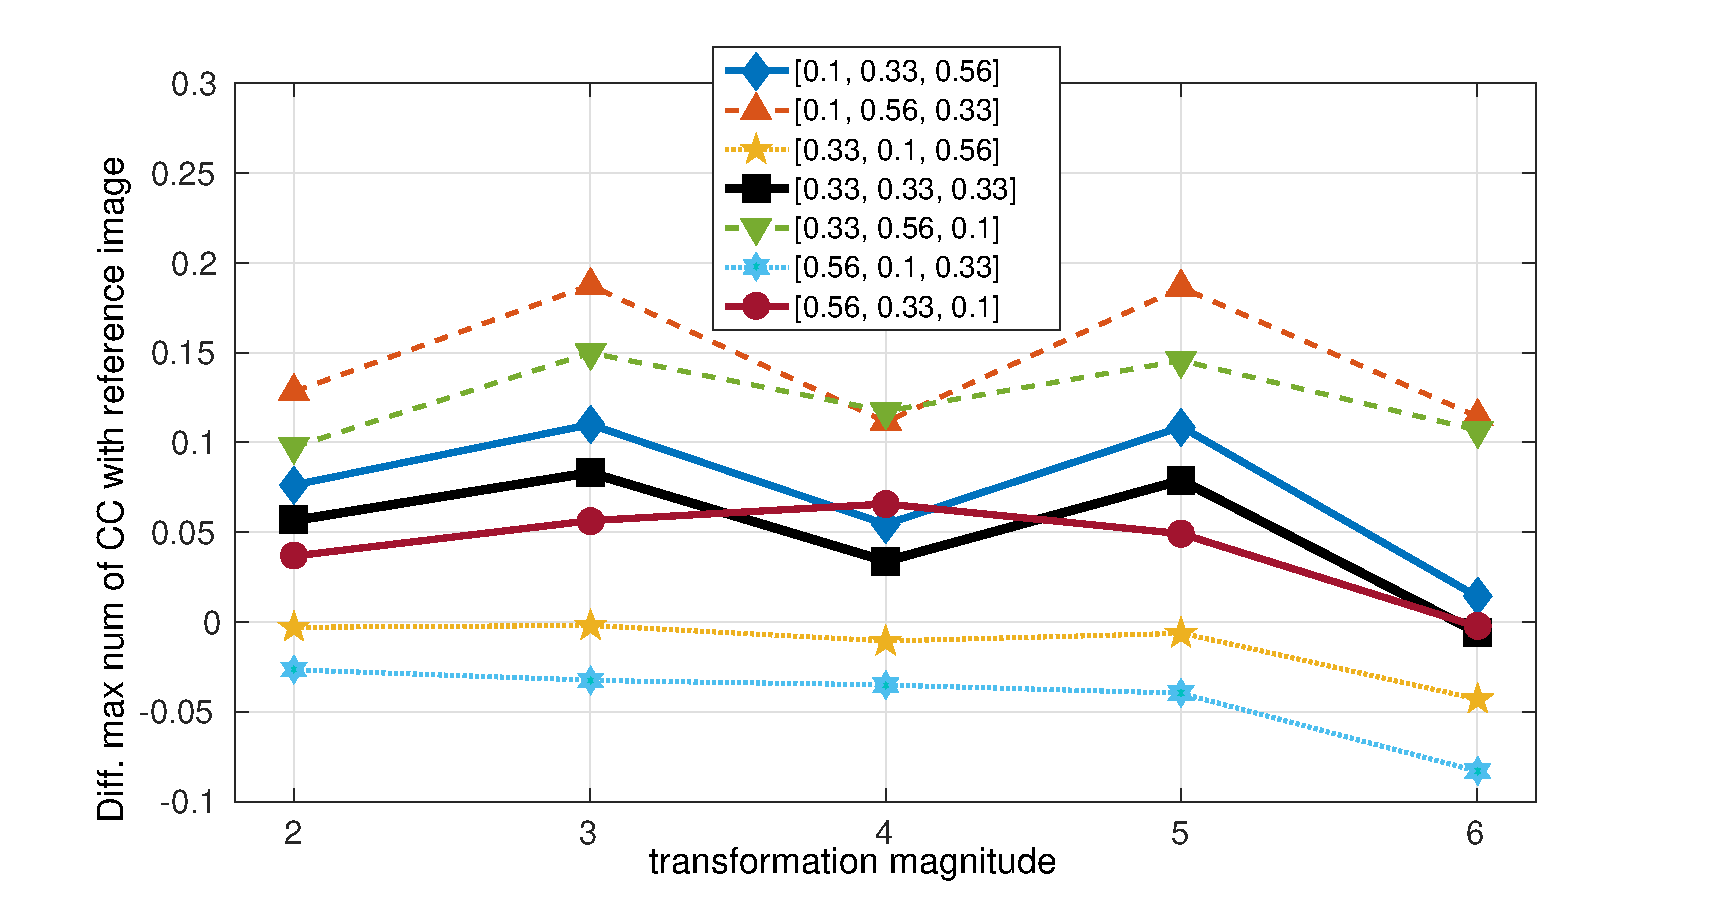
\includegraphics[width=8cm]{diff_num_cc_bin}}
 % \vspace{0.2cm}
 % \centerline{(a) MSER}\medskip
\end{minipage}
\hfill
%\vspace{-0.25cm}
\caption{Determining binarization weights. Difference between maximum number of CC for each pair of images (base, transf) for 7 weight combinations. Blur sequence ('Bikes'), Oxford dataset.}
\label{fig:bin_bikes}
%
\end{figure}

Figure \ref{fig:bin_bikes} shows several of the plots of the difference between the normalized maximum number of CC of the first reference image and each of the $5$ transformed images from the blur sequence 'Bikes', Oxford dataset, for several combinations of weights. Those configurations for which the differences are below $0$ are not desirable, since the number of CC decreases with the transformation. The combination of weights with the smallest and uniform positive differences and preferably small for the most extreme transformation (the $6$th image of the sequence) is preferred. After testing across all transformations, we have concluded that the most constant maximum number of CC is achieved when all weights are equal, i.e.  $w^{\cdot}=0.33$. 

%------------------------------------------------------------------------
\subsection{Oxford dataset}
\label{ssec:oxford}
Each image sequence of the Oxford dataset consists of one base and five increasingly distorted images \cite{Mikolajczyk:2005}. They are obtained independently of each other and the homographies between each pair $(\I_B,\I_T)$ are the provided  ground truth. Each sequence can be used to test only one transformation $T$. Therefore, it is not possible to separate transformation from image content. On the other hand, the Oxford dataset provides real homographies, unlike many other datasets.

For the viewpoint transformation ('Graffiti'), the best repeatability $R$ is achieved by DMSR with up to $72\%$ for a $40^{\circ}$ viewpoint change, which is $10\%$ more than the second performing MSER (Figure \ref{fig:rep_graffiti}). DMSR performs worse on the scale ('Boat'), but as well as or better than MSER on the blur ('Bikes', Fig.~\ref{fig:det_bikes}) and lighting ('Leuven') sequences \cite{elena_ranguelova_2016_45156}. These $R$ scores for all sequences of the dataset are achieved with consistently the smallest number of detected regions by DMSR, making the detector the most scaleable.  
%------------------------------------------------------------------------
\begin{figure}[htb]
\centering
\begin{minipage}[b]{.99\linewidth}
  \centering
  \centerline{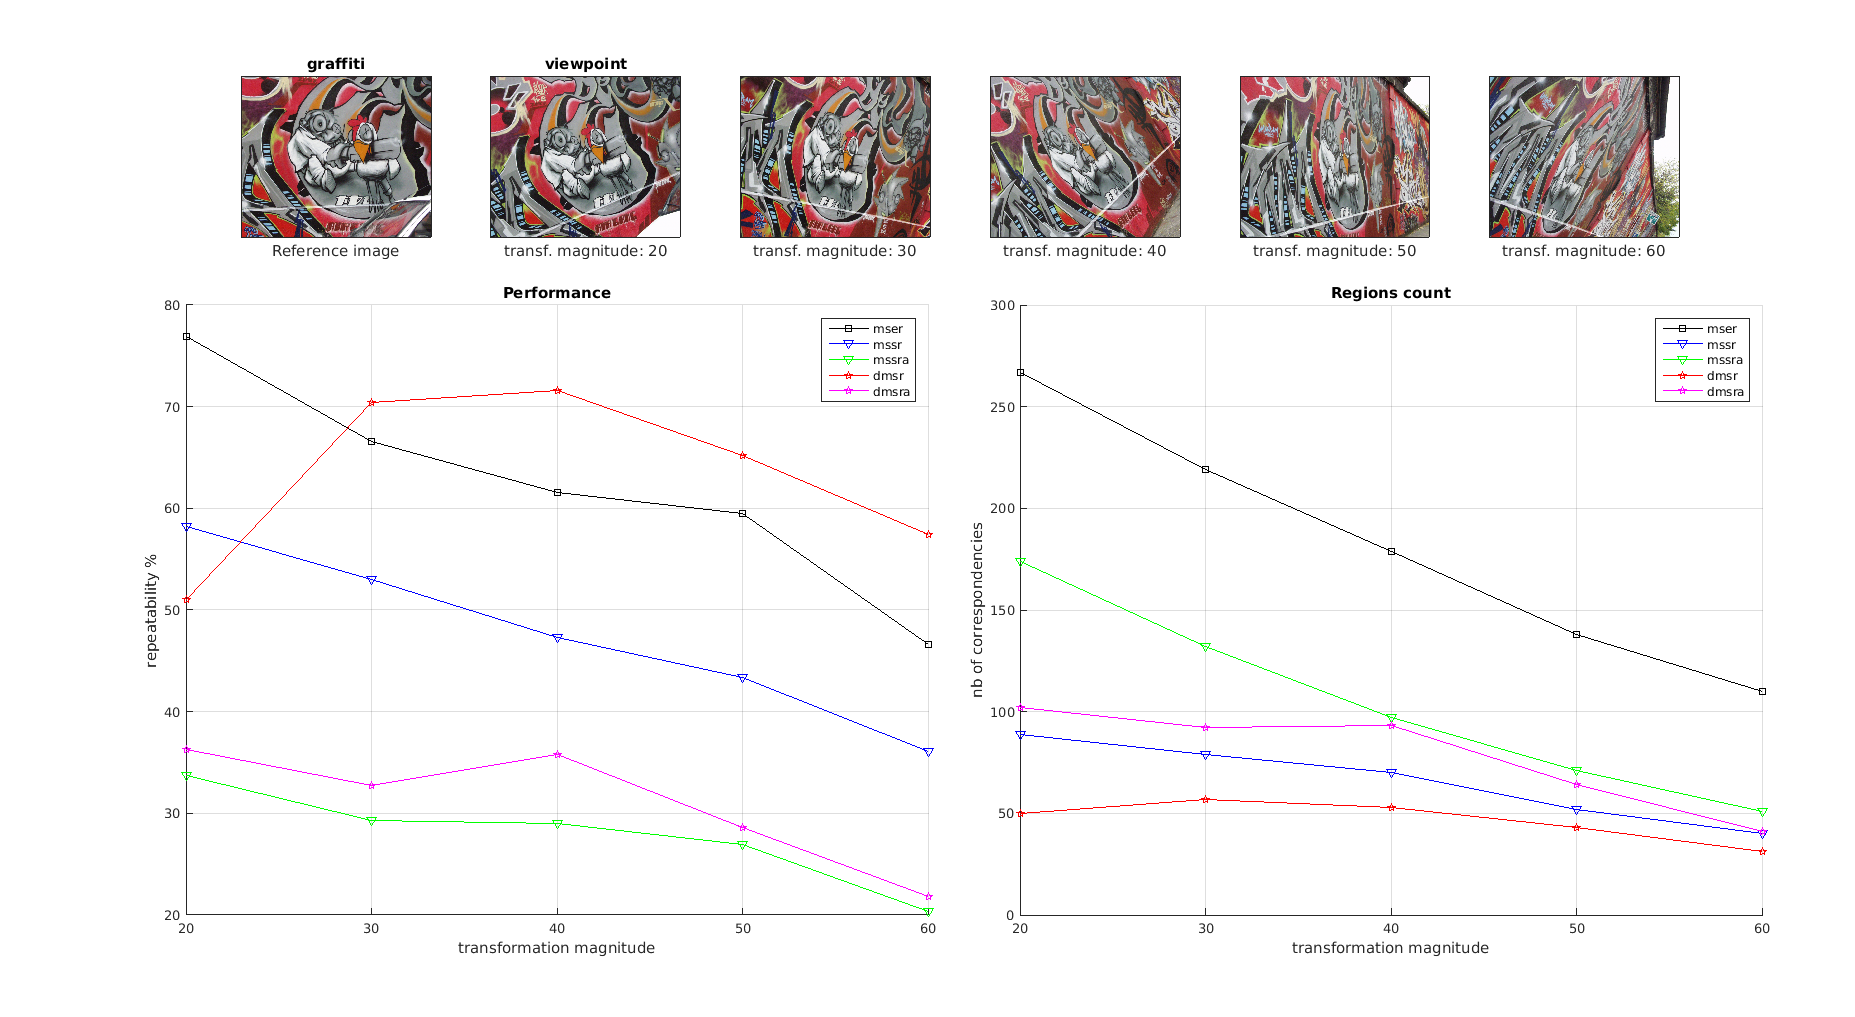
\includegraphics[width=8.5cm]{repeatability_all_affine_graffiti_viewpoint}}
 % \vspace{0.2cm}
 % \centerline{(a) MSER}\medskip
\end{minipage}
\hfill
%\vspace{-0.25cm}
\caption{Region detection on 'Graffiti', Oxford dataset.}
\label{fig:rep_graffiti}
%
\end{figure}
%------------------------------------------------------------------------
\begin{figure}[htb]
\centering
\begin{minipage}[b]{.99\linewidth}
  \centering
  \centerline{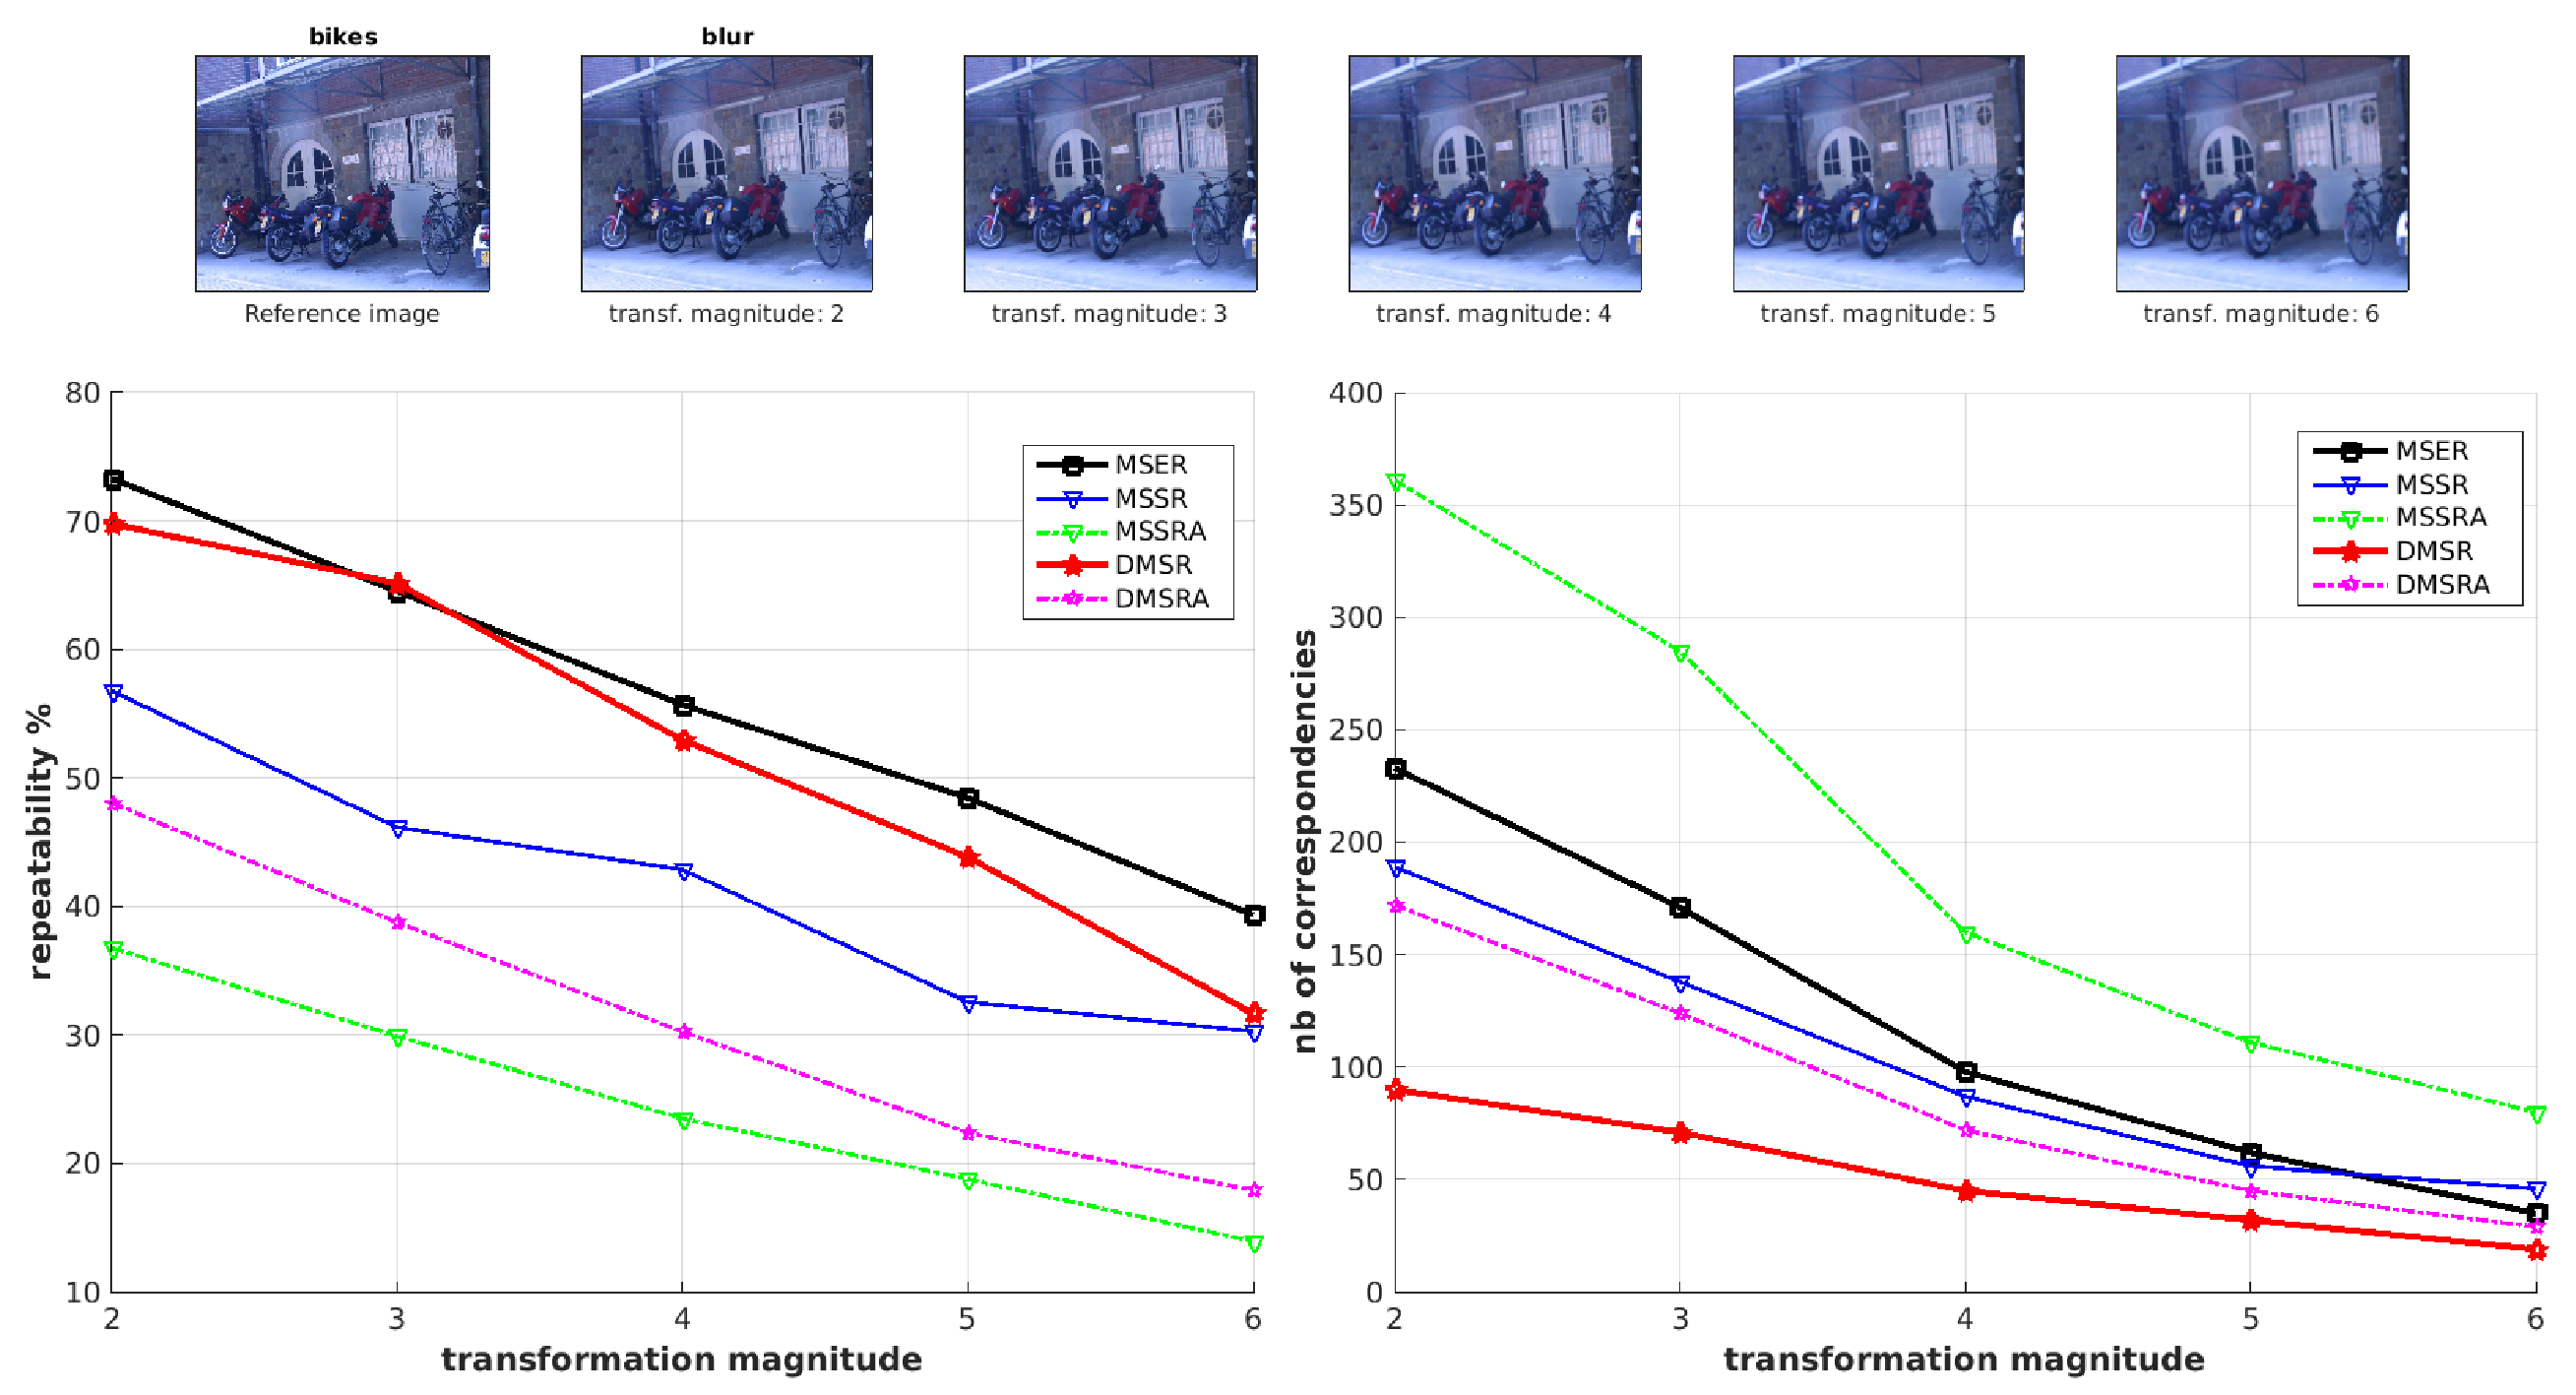
\includegraphics[width=8.5cm]{repeatability_all_affine_bikes_blur}}
 % \vspace{0.2cm}
 % \centerline{(a) MSER}\medskip
\end{minipage}
\hfill
%\vspace{-0.25cm}
\caption{Region detection on 'Bikes', Oxford dataset.}
\label{fig:det_bikes}
%
\end{figure}


\subsection{OxFrei dataset}
\label{ssec:combined}
A major drawback of the Oxford dataset is that one cannot determine whether the detector is robust to a transformation $T$, as every sequence represents only one $T$. The creators of the Freiburg dataset separated $T$ from the image content by applying a few transformations (alas not fully documented) to different base images \cite{FischerDB14}. To address the shortage of evaluation datasets, we have released OxFrei which combines the strong features of the Oxford and Freiburg datasets \cite{elena_ranguelova_2016_45156}. We have transformed the Freiburg base images with all homographies of the Oxford dataset. In this way, we have created $54$ images in $9$ structured scenes each under realistic blur, lighting, scaling and viewpoint transformations.

The dataset allows a transformation-independent robustness study by comparing performance on all data subject to the same realistic $T$. Figures~\ref{fig:det_frei} and \ref{fig:blur} show the $R$ score for lighting for one and blur for a few sequences. The standard plots (cf.~Fig.~\ref{fig:det_frei}) are cross-sections along the data dimension of the 3D plots (cf.~Fig.~\ref{fig:blur}) for one sequence. The 2D plots for all OxFrei experiments are available online \cite{elena_ranguelova_2016_45156}. From all experiments, we concluded that MSER is better for zoom and viewpoint (the latter contrasting with the result on the single Oxford 'Graffiti' sequence), while DMSR is robust to lighting and blur (Fig. \ref{fig:blur}). Again, the number of detected regions by DMSR is consistently the smallest across different image content and transformations.

%------------------------------------------------------------------------
%\vspace{-0.5cm}
\begin{figure}[htb]
\centering
\begin{minipage}[b]{.99\linewidth}
  \centering
 \centerline{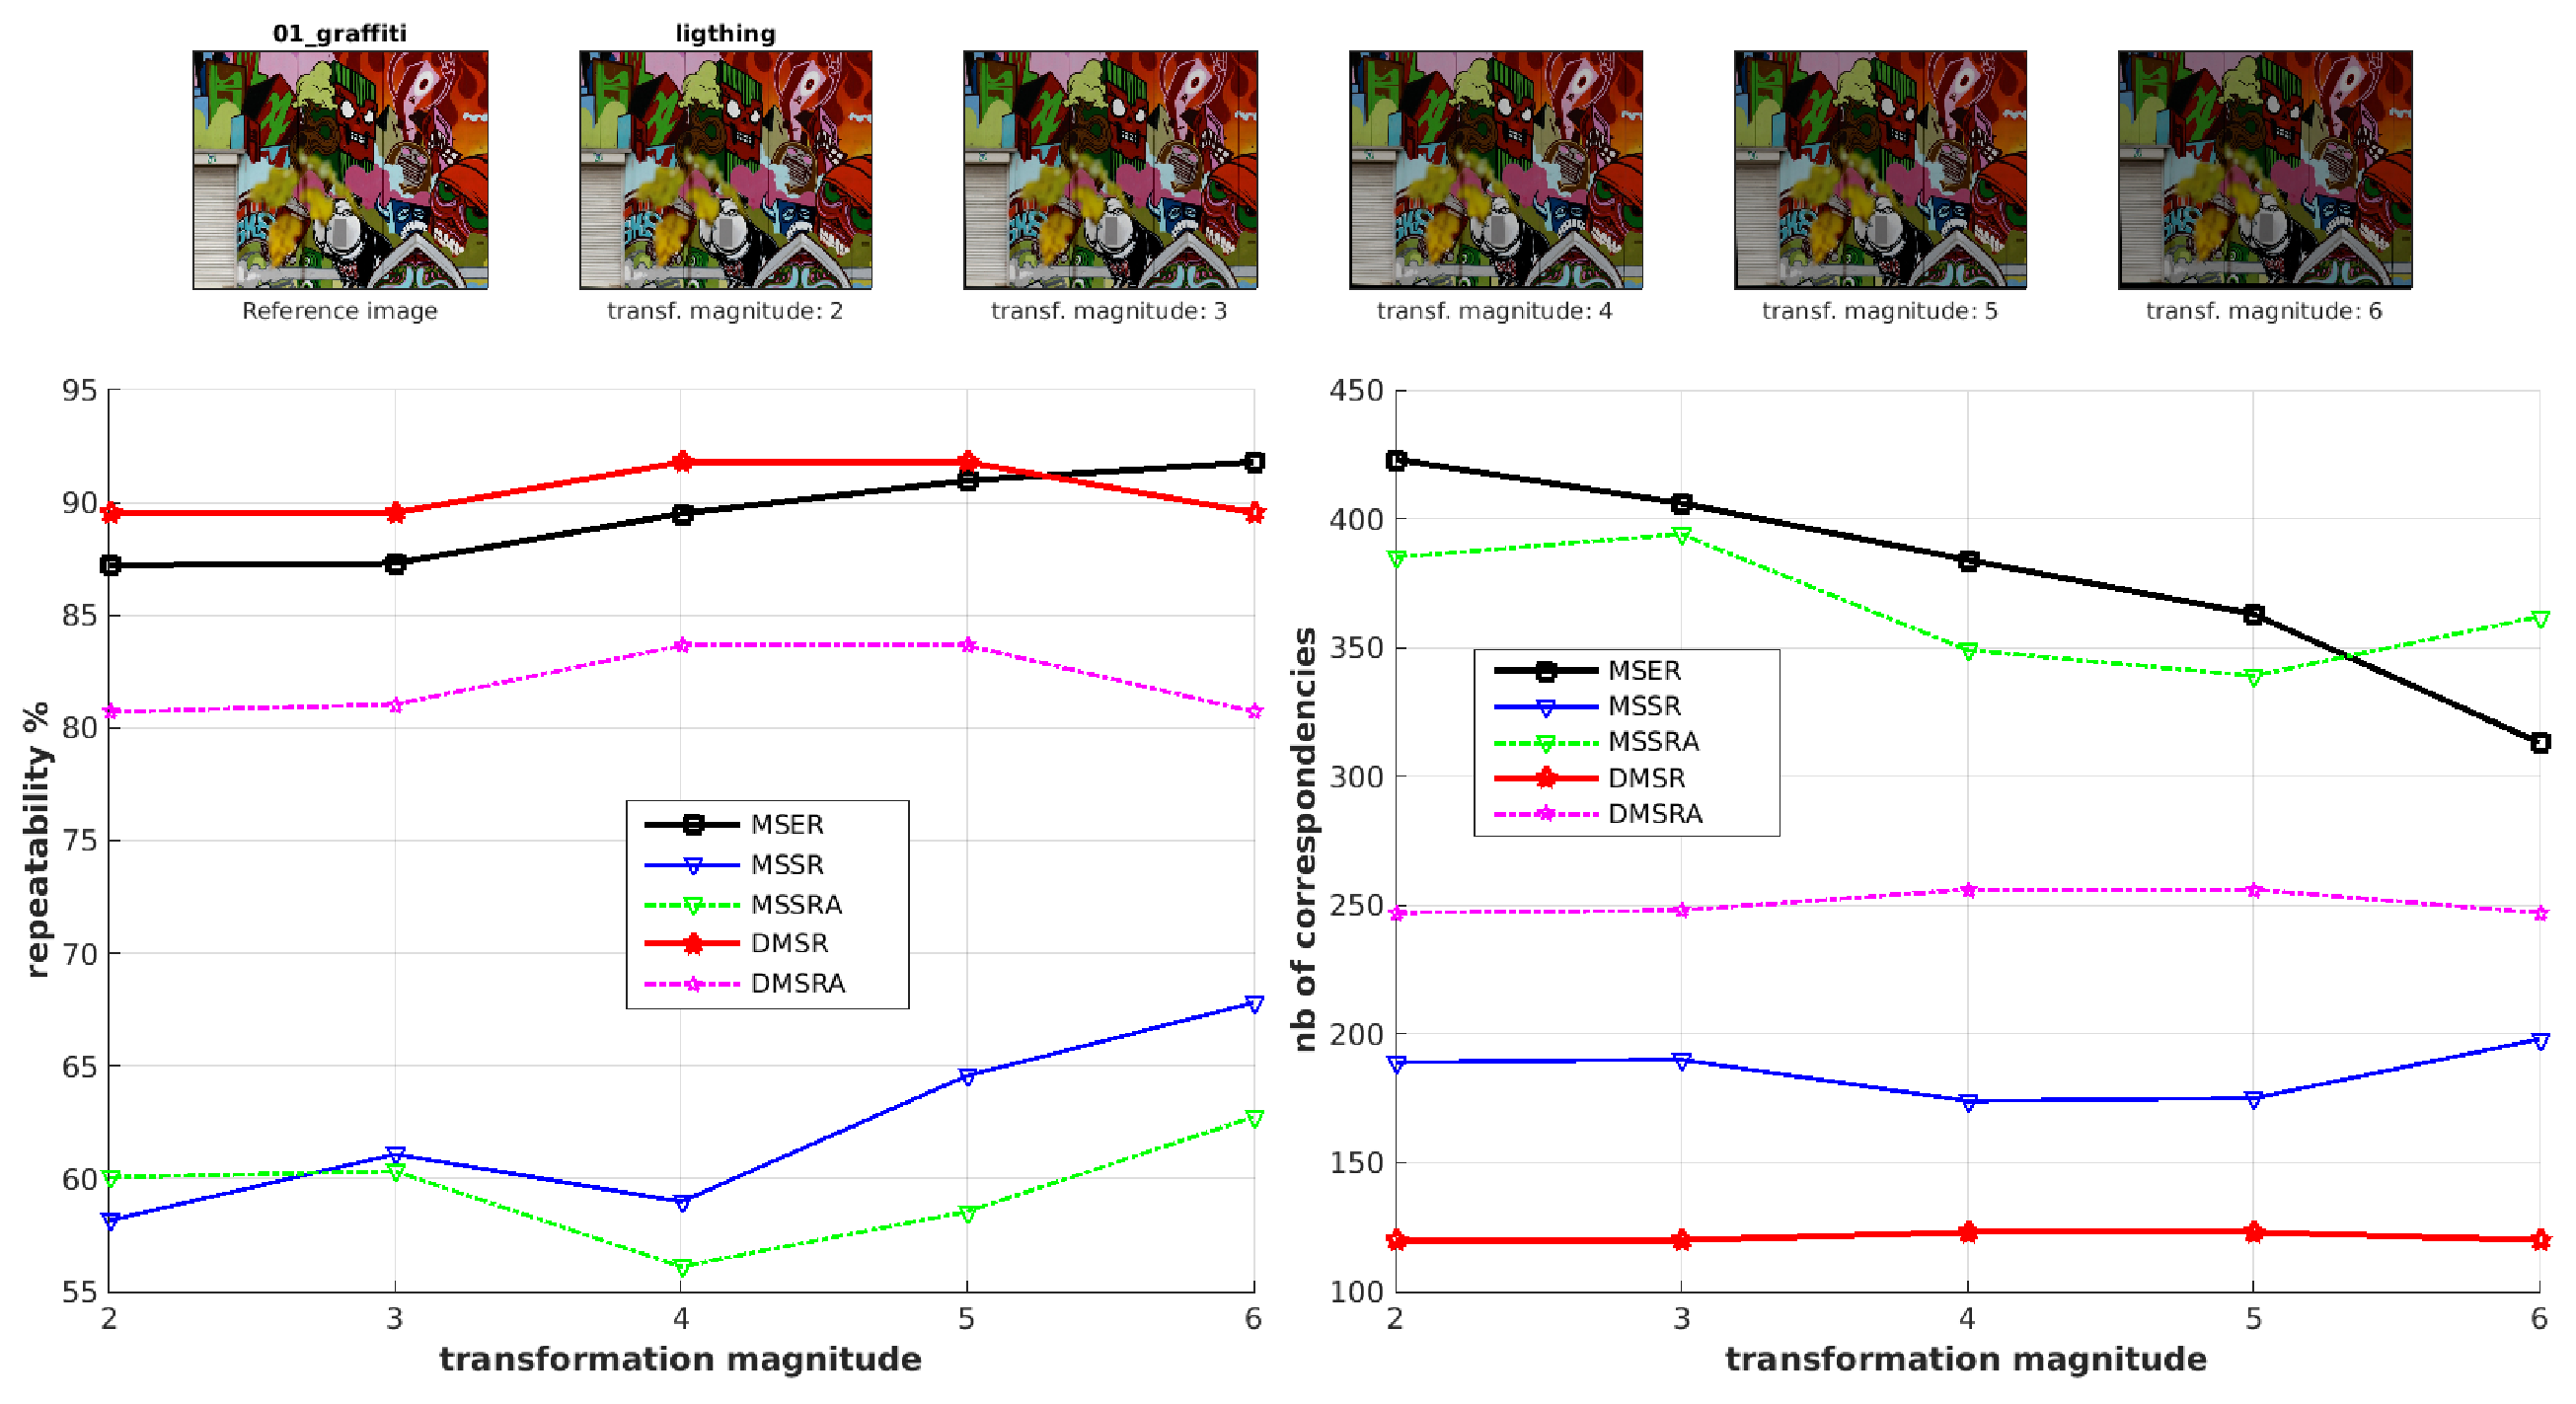
\includegraphics[width=8.5cm]{repeatability_all_combined_01_graffiti_ligthing_good}}
 % \vspace{0.2cm}
 % \centerline{(a) MSER}\medskip
\end{minipage}
\hfill
%\vspace{-0.25cm}
\caption{Region detection on '01\_graffiti', OxFrei dataset.}
\label{fig:det_frei}
%
\end{figure}
%------------------------------------------------------------------------

\begin{figure}[htb]

\begin{minipage}[b]{.9\linewidth}
  \centering
  \centerline{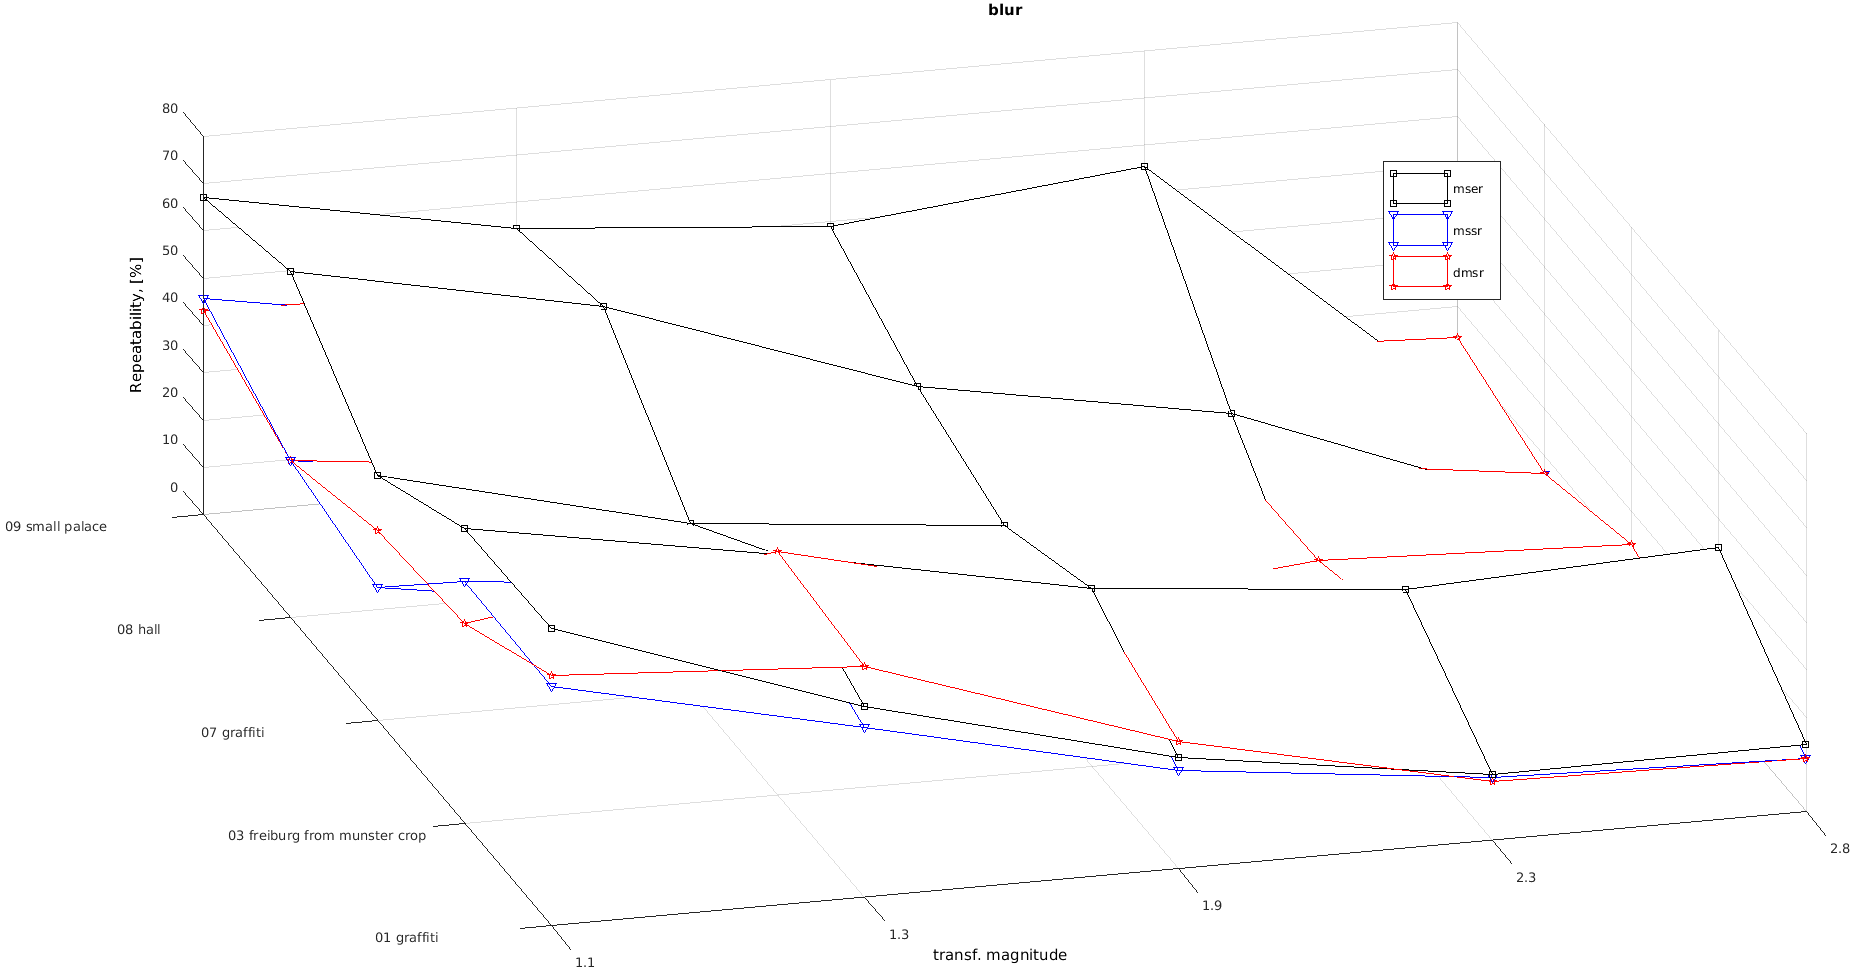
\includegraphics[width=8.5cm]{blur_some_combined}}
 % \vspace{0.2cm}
 % \centerline{(a) MSER}\medskip
\end{minipage}
\hfill
%\vspace{-0.25cm}
\caption{Robustness of region detectors to blur on five sequences of the OxFrei dataset.}
\label{fig:blur}
%
\end{figure}
%------------------------------------------------------------------------
\subsection{TNT hi-res benchmark}
\label{ssec:tnt}

The $R$ score of all detectors from the Oxford evaluation study drops on hi-res images \cite{CorRos2013}. On the 'underground' sequence from the TNT set, MSER loses up to $25\%$ between $1.5$~Mpx ($R_1$) and $8$Mpx ($R_4$) resolutions. On the contrary, DMSR increases the $R$ score as resolution increases on 'underground' and 'posters' sequences with up to $75\%$, which is a $15\%$ increase from $R_1$ to $R_4$ for a $40^{\circ}$ viewpoint change (Figure \ref{fig:tnt}). We can even observe that easily by qualitative inspection of the actual detected regions as we already have shown on Figure \ref{fig:tnt_zoom}. While MSER increasinly loses features as the image resolution increases, the number and location of DMSR regions remains stable.

\begin{figure}[htb]

\begin{minipage}[b]{.9\linewidth}
  \centering
  \centerline{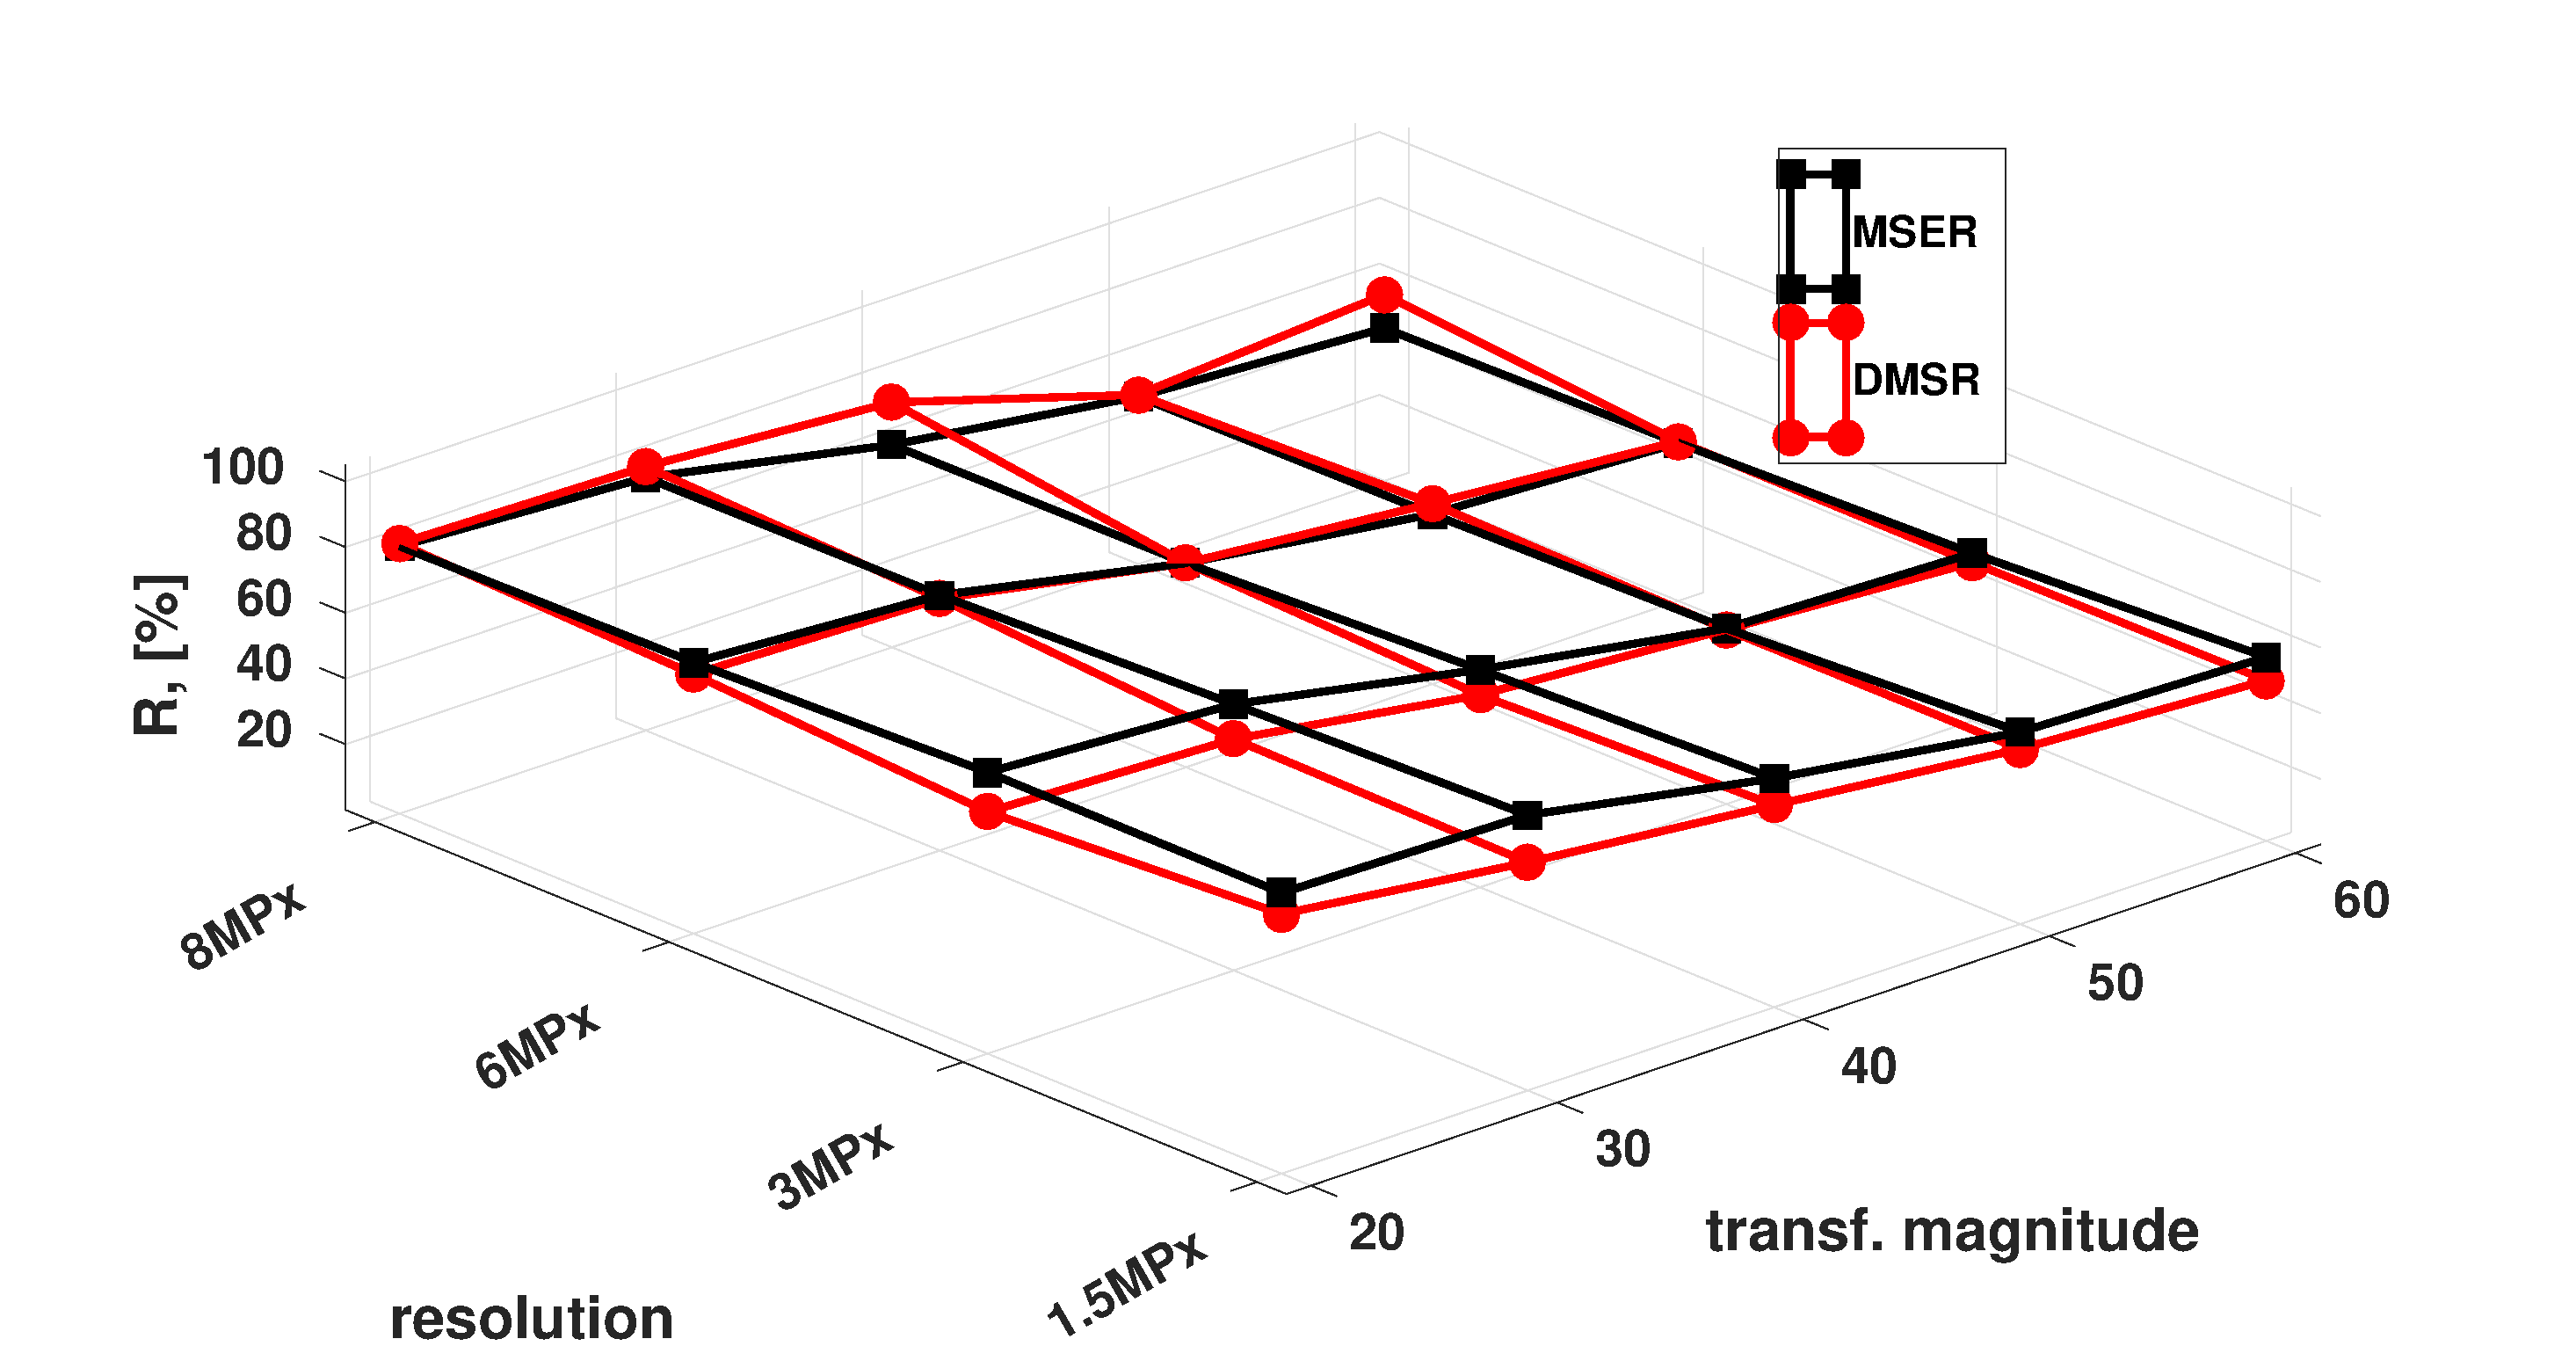
\includegraphics[width=8.5cm]{posters_rep}}
 % \vspace{0.2cm}
 % \centerline{(a) MSER}\medskip
\end{minipage}
\hfill
\caption{Robustness of region detectors to image resolution and viewpoint. 'Posters', TNT dataset.}
\label{fig:tnt}
\vspace{-0.25cm}
\end{figure}
%------------------------------------------------------------------------
\begin{figure}[htb]

\begin{minipage}[b]{0.9\linewidth}
  \centering
  \centerline{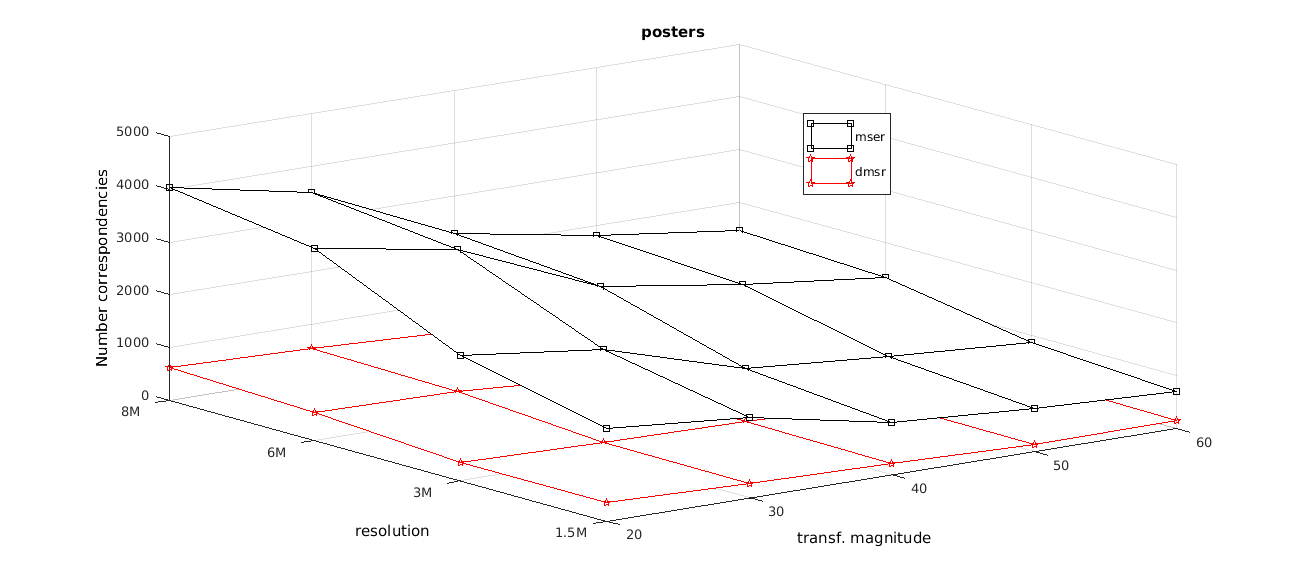
\includegraphics[width=8.5cm]{posters_numreg}}
 % \vspace{0.2cm}
 % \centerline{(b) DMSR}\medskip
\end{minipage}
%\vspace{-0.25cm}
\caption{Number of region correspondences versus image resolution and viewpoint. 'Posters', TNT dataset.}
\label{fig:tnt_numreg}
%
\end{figure}
%------------------------------------------------------------------------

Again, the $N_C$ plane of DMSR has the lowest values and the smallest slope of all detectors (Figs.~\ref{fig:rep_graffiti}, \ref{fig:det_bikes}, \ref{fig:det_frei}, right and Fig.~\ref{fig:tnt_numreg} and \cite{elena_ranguelova_2016_45156}). The number of detected DMSR regions is up to an order of magnitude lower compared to MSER - crucial for the efficiency of the following matching step on large-scale image datasets.

\subsection{Animal and plant biometrics}
\label{ssec:bio}
Challenged by the photo-identification and phenotypical measurement tasks of ecologists, we aimed to test if our detector is able to solve both problems. Photo-identification of individuals or species involves the comparision of a new image to the exsisting catalogue of known individuals or species, similar to many generic applications. Phenotypic measurements invole the computation of properties of (exact-shaped) regions with semantic meaning.

Due to the lack of openly accessible large-scale annotated animal or plant biometric datasets, we performed only preliminary experiments on few small datasets, from which we could gain some insights into the performance of the detector. We have qualitatively compared DMSR and MSER on several small animal individual photo-ID datasets (humpback whales, leatherback turtles, newts) and on a wood species identification dataset \cite{RangHumpb06, PauwelsZB08, wood}. 

In all cases, DMSR produced fewer and perceptually more acurate salient regions, as illustrated by Figures~\ref{fig:tails_mser}, \ref{fig:tails_dmsr}, \ref{fig:turtle} and \ref{fig:wood}, \ref{fig:wood_C}. For some of the leatherback turtles, the MSER did not find any or very few regions, which will make the subsequent matching for photo-identification impossible. On the other hand, the DMSR regions were detected consistently and repeatedly (Fig.~\ref{fig:turtle}). For the wood microscopy images, we observed that it is not possible to obtain accurate statistics on the cell properties using the regions from the MSER detector, while the regions found by our detector would enable such wood anatomy research (Fig.~\ref{fig:wood}, \ref{fig:wood_C}). Also, we used the exact shapes of the detected regions to compute the wood cell properties (such as size, eccentricity and orientation) using those for successful classification of $19$ images into $9$ wood species \cite{elena_ranguelova_wood}. 

Another advantage of DMSR is the option to selectively detect only some types of salient regions (unlike MSER or any other detector) in which the ecologists are interested. In the wood microscopy images only the light cells are of interest and hence we can chose only to detect 'islands'. Using all $4$ types of regions does not seem to improve performance over using only $ISS$ (holes and islands), with the exception of detecting markings on humpback whale tails (Figs.~\ref{fig:tails_mser}, \ref{fig:tails_dmsr}). 

\begin{figure}[htb]

\begin{minipage}[b]{.99\linewidth}
  \centering
  \centerline{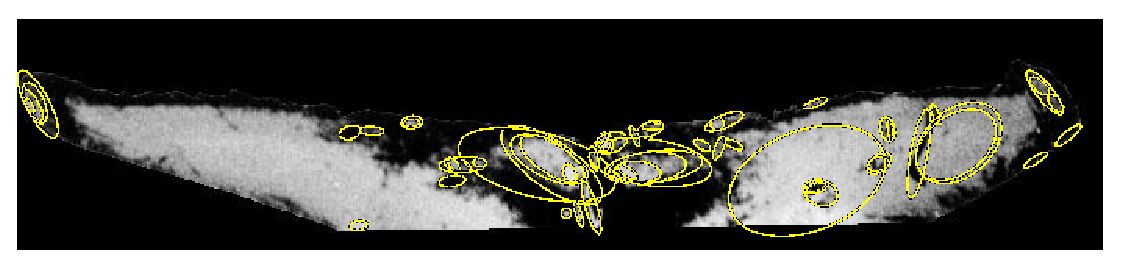
\includegraphics[width=8cm]{mserTailA}}
\end{minipage}
\vspace{0.1cm}
\begin{minipage}[b]{0.99\linewidth}
  \centering
  \centerline{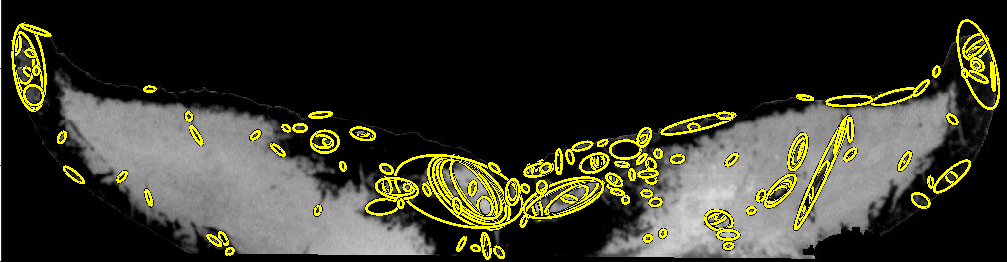
\includegraphics[width=8cm]{mserTailB}}
\end{minipage}
\hfill
%\vspace{-0.4cm}
\caption{MSER detection on two images of the tail of a humpback whale. }
\label{fig:tails_mser}
\vspace{-0.3cm}
\end{figure}

\begin{figure}[htb]

\begin{minipage}[b]{.99\linewidth}
  \centering
  \centerline{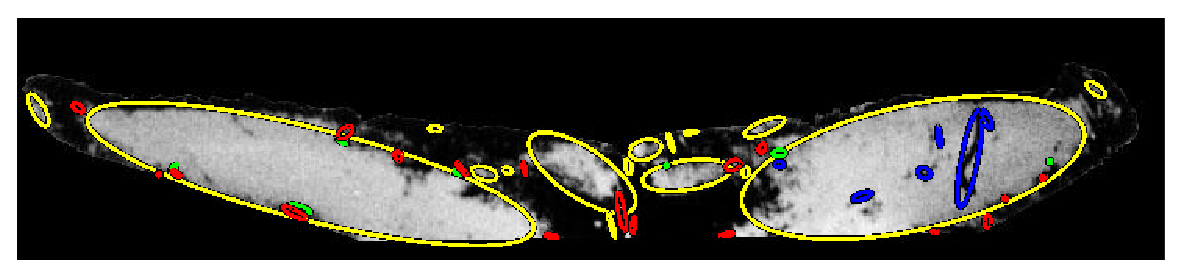
\includegraphics[width=8cm]{dmsrTailA}}
\end{minipage}
\vspace{0.1cm}
\begin{minipage}[b]{0.99\linewidth}
  \centering
  \centerline{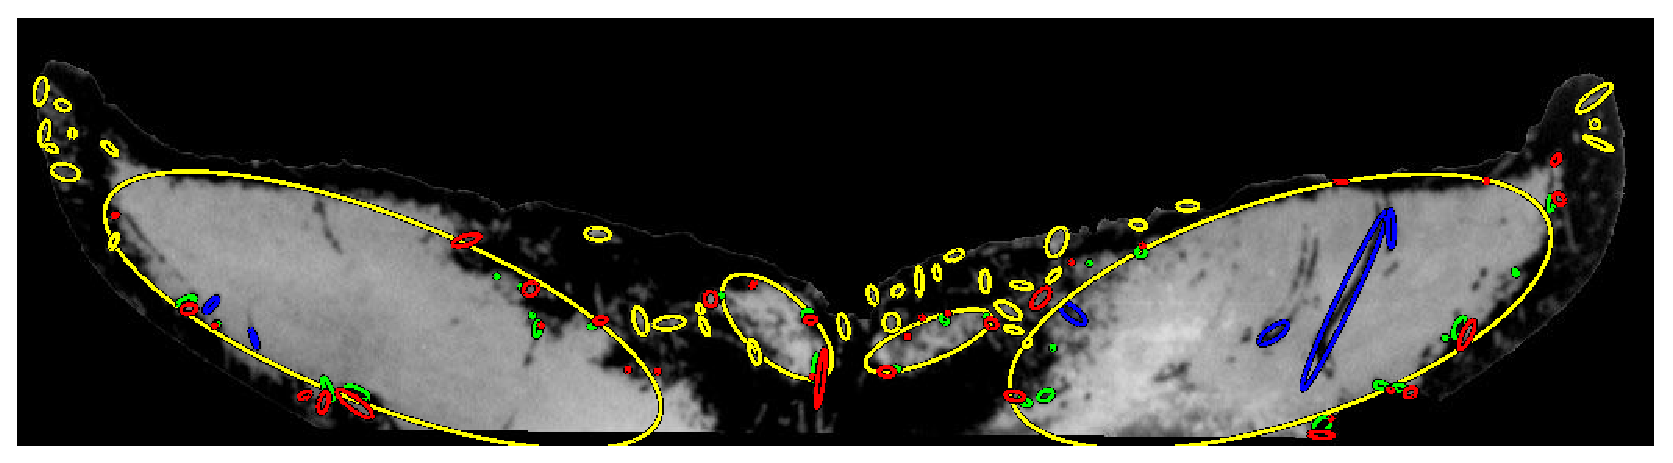
\includegraphics[width=8cm]{dmsrTailB}}
\end{minipage}
\hfill
%\vspace{-0.4cm}
\caption{DMSRA detection on two images of humpback whale tail. The salient region types are color-coded like on Fig.~\ref{fig:binary_sal}}
\label{fig:tails_dmsr}
\vspace{-0.3cm}
\end{figure}

\begin{figure}[htb]

\begin{minipage}[b]{.23\linewidth}
  \centering
  \centerline{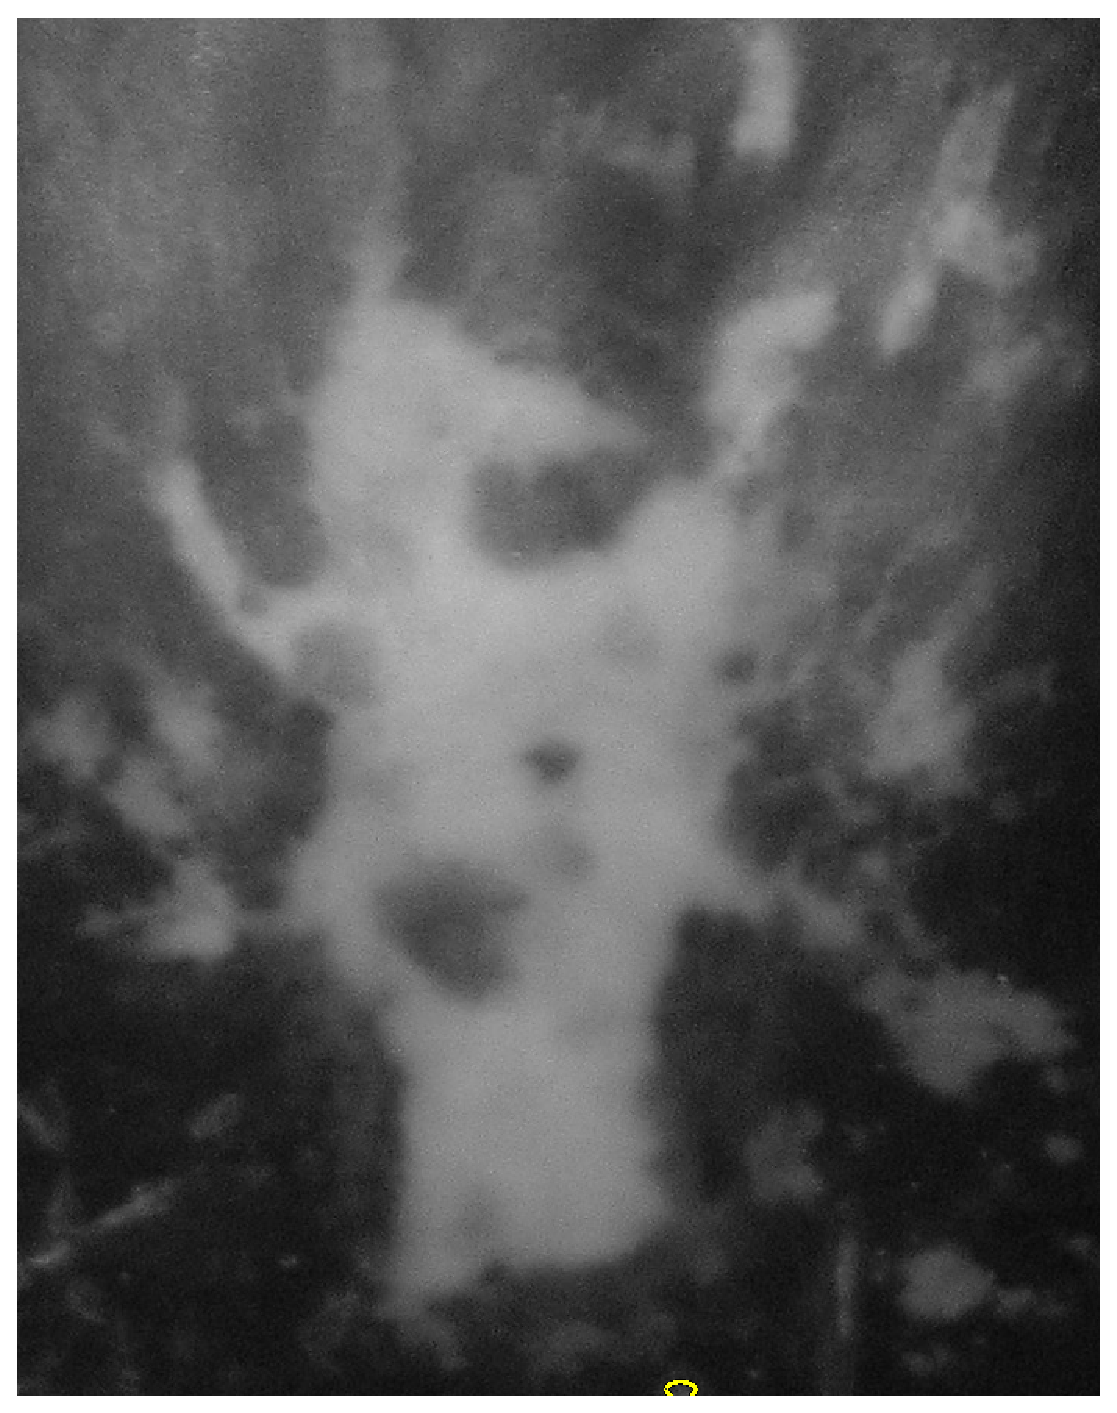
\includegraphics[width=1.8cm]{mserLeatherbackA}}
   \centerline{(a)}\medskip
\end{minipage}
\hfill
\begin{minipage}[b]{0.23\linewidth}
  \centering
  \centerline{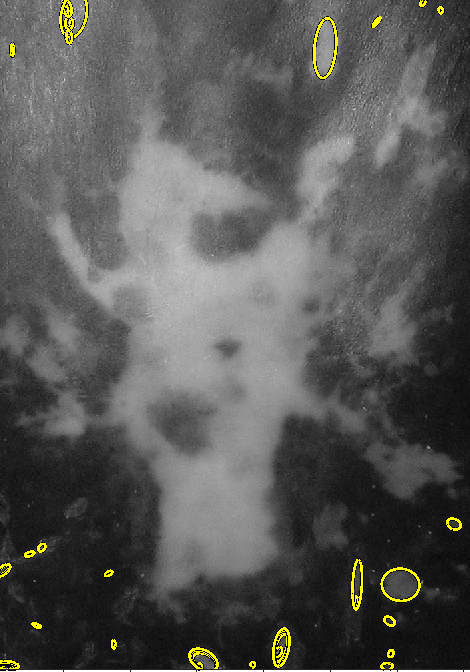
\includegraphics[width=1.8cm]{mserLeatherbackB}}
\centerline{(b)}\medskip
\end{minipage}
\hfill
\begin{minipage}[b]{.23\linewidth}
  \centering
  \centerline{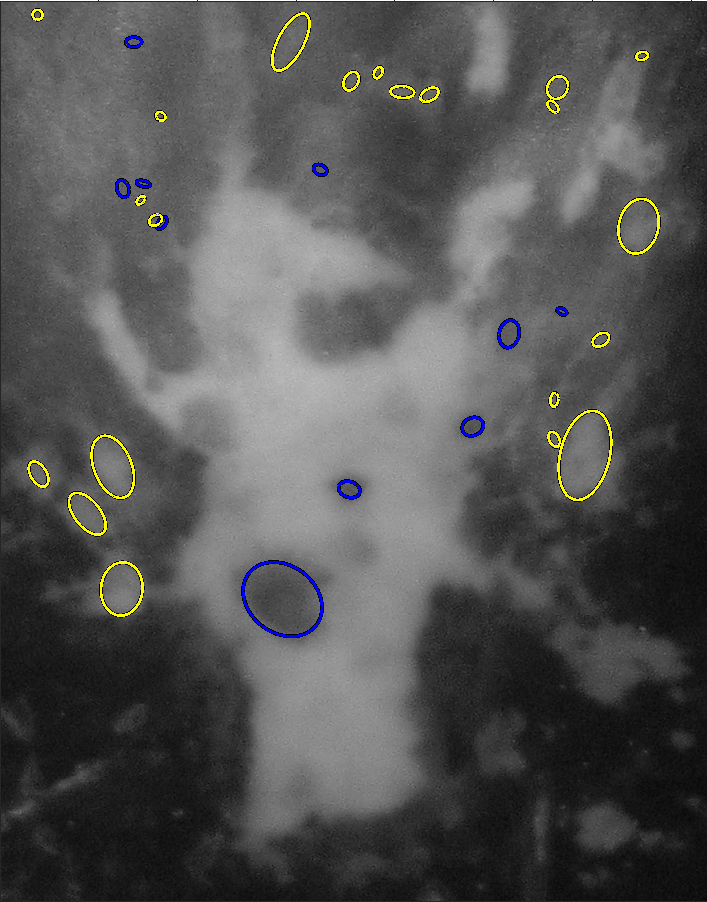
\includegraphics[width=1.8cm]{dmsrLeatherbackA}}
\centerline{(c)}\medskip
\end{minipage}
\hfill
\begin{minipage}[b]{0.23\linewidth}
  \centering
  \centerline{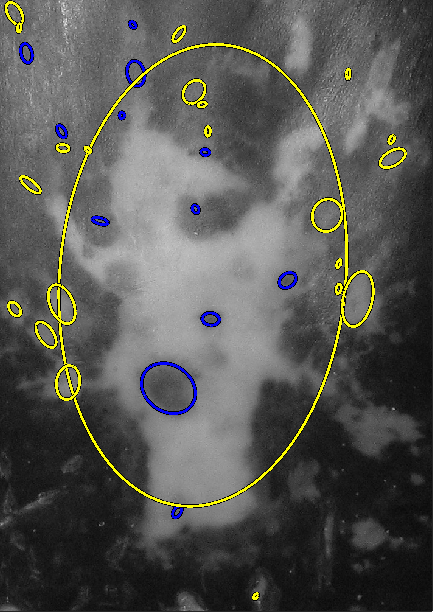
\includegraphics[width=1.8cm]{dmsrLeatherbackB}}
 \centerline{(d)}\medskip
\end{minipage}
 \vspace{-0.2cm} 
\caption{Region detection on two images of the pineal spot of the same leatherback turtle.
(a),(b): MSER, (c),(d): DMSR. Note the lack of relevant regions in (a).}
\label{fig:turtle}
 \vspace{-0.2cm}
\end{figure}

 
\begin{figure}[htb]
\begin{minipage}[b]{.99\linewidth}
  \centering
  \centerline{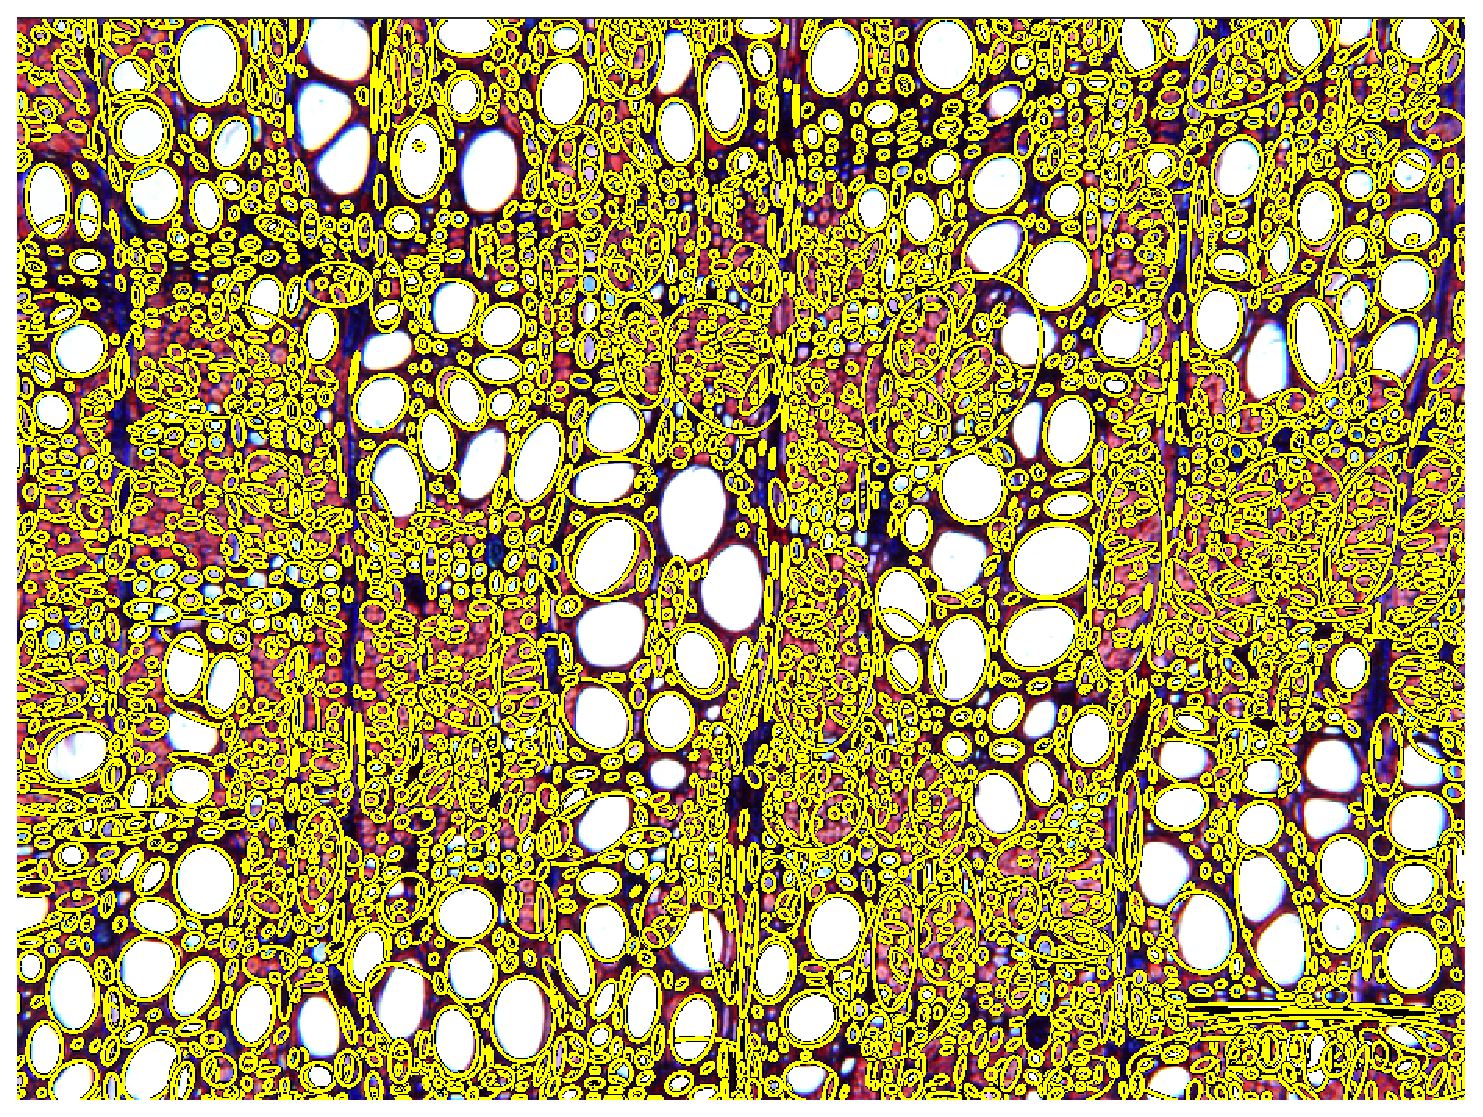
\includegraphics[width=6cm]{mserWood}}
\end{minipage}
\hfill
\vspace{0.2cm}
\begin{minipage}[b]{0.99\linewidth}
  \centering
  \centerline{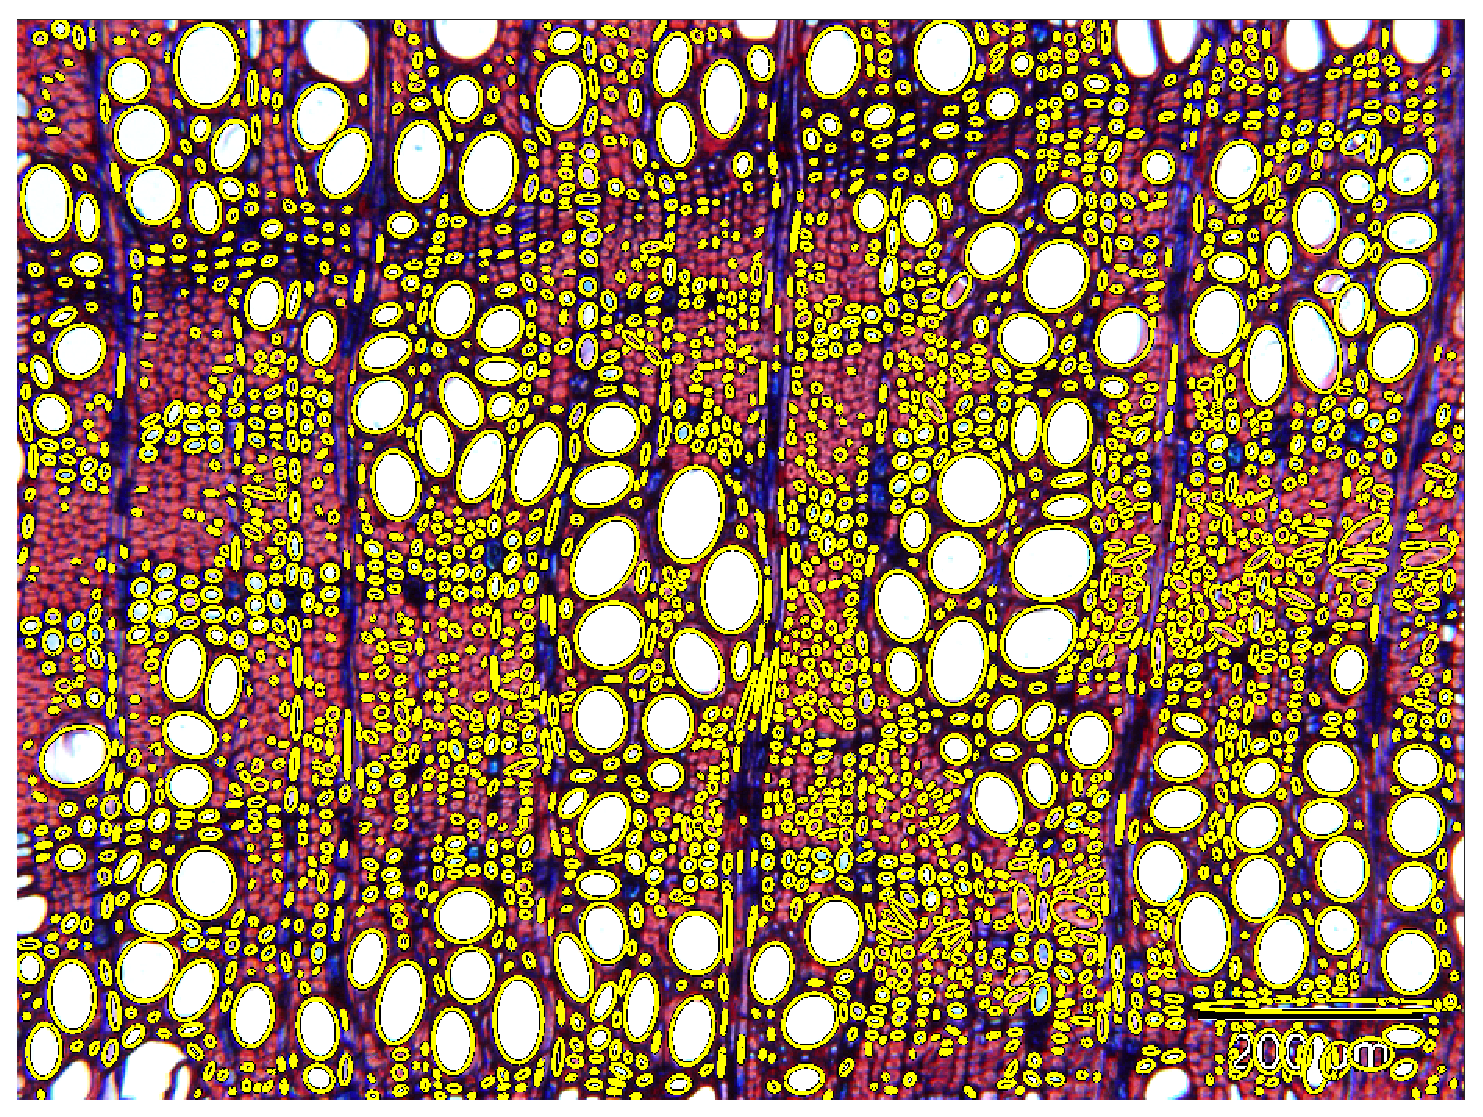
\includegraphics[width=6cm]{dmsrWood}}
\end{minipage}
\vspace{-0.1cm}
\caption{Salient region detectors on microscopy wood (Argania spinosa) image. Elliptic representation. Top: MSER (every second region is shown), bottom: DMSR}
\label{fig:wood}
\end{figure}
%\vspace{-0.3cm}

\begin{figure}[htb]
\begin{minipage}[b]{.49\linewidth}
  \centering
  \centerline{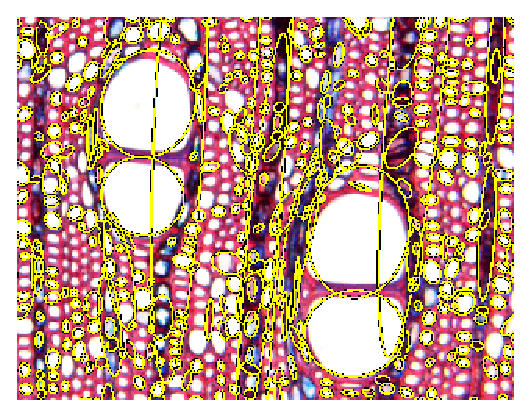
\includegraphics[width=4cm]{mser_wood_C}}
\end{minipage}
\hfill
\begin{minipage}[b]{0.49\linewidth}
  \centering
  \centerline{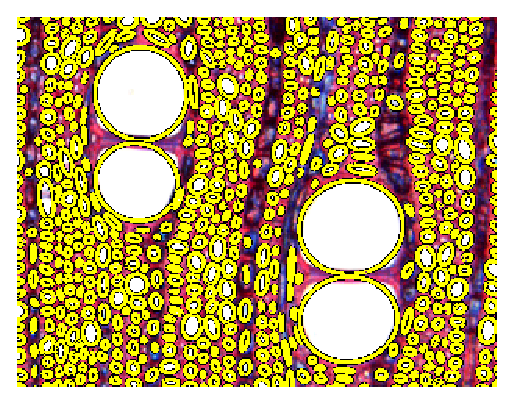
\includegraphics[width=4cm]{dmsr_wood_C}}
\end{minipage}
\vspace{-0.25cm}
\caption{Salient region detectors on microscopy wood (Chrys afr) image (detail). Elliptic representation. Left: MSER (every $3$rd region is shown), right: DMSR}
\label{fig:wood_C}

\end{figure}
%\pagebreak
%%%%%%%%%%%%%%%%%%%%%%%%%%%%%%%%%%%%%%%%%%%%%%%%%%%%%%%%%%%%%%%%%%%%%%%%%%%%%%%%%%%%%%%%%%%%%%%%%%%%%%%%%%%%%%%%%%%%%%%%%%%%%%%%%%%%%%%%%%%%%%%%%%%%%%%%%%%%%%%%%%%%%%%%%

\section{Conclusion}

Combining data-driven binarization with morphological operations yields a region detector with comparable to superior performance to MSER on various datasets. DMSR produces a much smaller number of regions - a much desired property in large-scale processing. It can cope better with blur, lighting and increased resolution. Furthermore, it detects semantically meaningful salient regions, which makes it a promising candidate for scientific imagery analytics, especially for the photo-identification and phenotypic measurement tasks. For detection evaluation, high-resolution transformation-independent datasets, like the OxFrei we introduced, should become the standard. In our future work, we plan to formally evaluate the completeness of the DMSR detector and to run extensive validation experiments on large-scale animal and plant biometric datasets.

% use section* for acknowledgment
\ifCLASSOPTIONcompsoc
  % The Computer Society usually uses the plural form
  \section*{Acknowledgments}
\else
  % regular IEEE prefers the singular form
  \section*{Acknowledgment}
\fi
The authors would like to thank Frederic Lens from the Naturalis biodiversity institute in Leiden, Netherlands, for providing the wood microscopy images \cite{wood}.


% references section

% can use a bibliography generated by BibTeX as a .bbl file
% BibTeX documentation can be easily obtained at:
% http://mirror.ctan.org/biblio/bibtex/contrib/doc/
% The IEEEtran BibTeX style support page is at:
% http://www.michaelshell.org/tex/ieeetran/bibtex/
%\bibliographystyle{IEEEtran}
% argument is your BibTeX string definitions and bibliography database(s)
%\bibliography{IEEEabrv,../bib/paper}
%
% <OR> manually copy in the resultant .bbl file
% set second argument of \begin to the number of references
% (used to reserve space for the reference number labels box)

\bibliographystyle{IEEEtran}
\bibliography{aiccsa2016}


% that's all folks
\end{document}


